\chapter{Methodology}\label{ch:methodology}

This chapter describes how the research was conducted, from ECG data preparation
to evaluation of the frozen classification system. Section~\ref{ch:data}
defines the datasets, annotation groups, and allocation of examples.
Section~\ref{ch:theory} explains the theoretical basis of the signal features
and learning algorithms. Section~\ref{ch:architecture} specifies the implemented
models and their computational operations. Section~\ref{sec:method-training-inference}
then follows training and inference mathematically, using small worked
calculations and an end-to-end case study with real ECG segments.
Finally, Section~\ref{ch:method} defines the experimental design, evaluation
populations, metrics, and uncertainty analysis used for the results in
Chapter~\ref{ch:results}.

\section{Data and preparation}\label{ch:data}

This section identifies the ECG sources, explains how the signals are
prepared, and shows how examples enter model fitting, validation, and the
temporal test. Keeping these roles separate prevents healthy data or test
labels from being used in the wrong part of the study.

\subsection{Data sources and roles}

Two public PhysioNet databases supply model development data. A separate,
limited external INCART check is reported in the results chapter. The MIT--BIH Normal Sinus Rhythm
Database (NSRDB) supplies normal-reference ECG for the autoencoder. The MIT--BIH
Arrhythmia Database (MITDB) supplies labelled normal and abnormal beats for the
detector, subtype classifier, and final temporal evaluation
\cite{goldberger2000physionet,nsrdb,mitdb}.

\begin{table}[H]
\centering
\small
\caption{Data sources and their strictly separated roles.}
\label{tab:data-source-role}
\begin{tabular}{@{}>{\raggedright\arraybackslash}p{2.6cm}>{\raggedright\arraybackslash}p{3.8cm}>{\raggedright\arraybackslash}p{4.8cm}@{}}
\toprule
Source & Available data & Use in this study\\
\midrule
\makecell[l]{MIT--BIH\\Normal Sinus\\Rhythm DB\\(NSRDB)} &
18 real long-term ECG recordings from five men aged 26--45 and 13 women aged
20--50, with no significant arrhythmias; two stored channels named ECG1 and
ECG2; 128 Hz; approximately 23--26 hours per record \cite{nsrdb}. &
The complete first stored ECG channel from every record is processed. Fifteen
subjects fit the normal-only autoencoder and three different subjects validate
it and determine the normal residual threshold.\\
\addlinespace
\makecell[l]{MIT--BIH\\Arrhythmia DB\\(MITDB)} &
48 approximately 30-minute, two-channel ambulatory ECG records from 47
subjects (25 men aged 32--89 and 22 women aged 23--89), sampled at 360 Hz,
with expert beat and rhythm annotations \cite{mitdb,moody2001impact}. &
Only the 46 records containing MLII are eligible. Their earlier 80\% supplies
supervised development and their final 20\% supplies the temporal test. These
records represent 45 subject clusters because records 201 and 202 belong to
one person.\\
\bottomrule
\end{tabular}
\end{table}

Figure~\ref{fig:data-source-overview} summarises these roles. NSRDB supplies
normal-reference windows for the autoencoder, while MITDB supplies labelled
MLII beats for supervised development and temporal testing.

\begin{figure}[H]
\centering
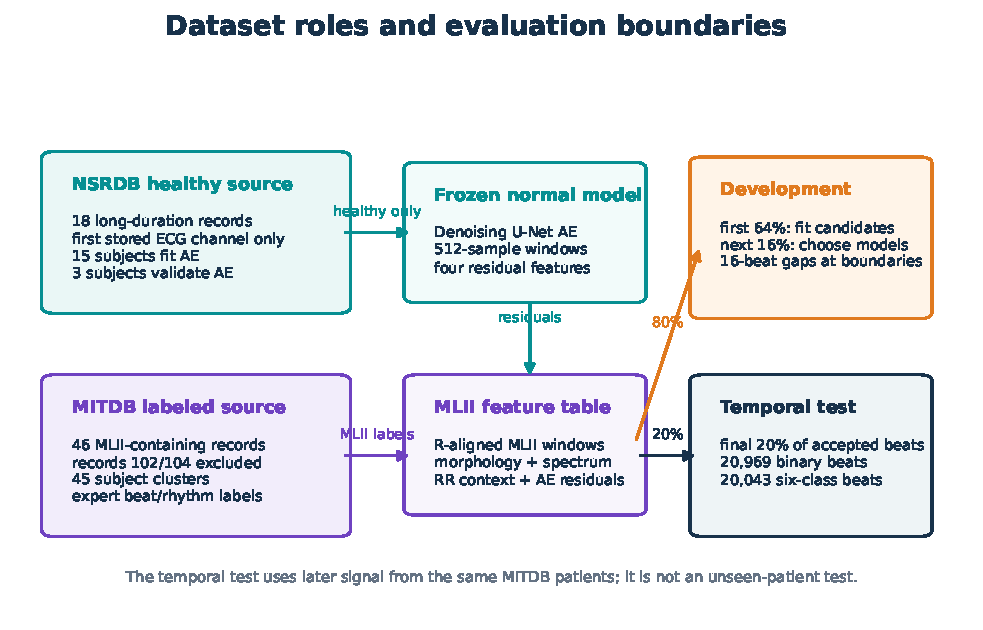
\includegraphics[width=.98\textwidth]{pic/generated/dataset_role_overview.pdf}
\caption{Dataset roles and evaluation boundaries. The healthy NSRDB channel
creates the frozen normal model. MITDB MLII creates the supervised feature table
and is split chronologically into development and temporal-test regions.}
\label{fig:data-source-overview}
\end{figure}

\textbf{Why NSRDB is used for healthy training.}
NSRDB contains real long-duration ECG from subjects reported to have no
significant arrhythmias. This matches the autoencoder idea: the network sees
normal structure without supervised arrhythmia labels. This is a nominally
normal source cohort, not an annotation-verified guarantee that every window
is normal. The preparation code does not exclude windows using NSRDB beat
annotations. All 18 subjects
and their complete recordings enter the cleaning process, giving 437.49 hours
of source ECG. Complete recordings also expose the model to normal within-day
variation instead of a short selected excerpt.

\textbf{Exactly one channel is used.}
NSRDB headers call the two waveforms ECG1 and ECG2; they do not identify either
as a standard anatomical lead. This study therefore selects the first stored
channel consistently and describes it as the \emph{first NSRDB ECG channel}.
It is not renamed Lead II. The second channel never enters autoencoder fitting,
validation, threshold estimation, or residual calculation.

The supervised branch uses MLII only. Modified Lead II is a bipolar torso
lead with a negative RA-equivalent electrode on the right upper torso and a
positive LL-equivalent electrode on the left lower torso. Figure~\ref{fig:data-lead-positions}
shows this polarity schematically; the separate reference electrode is shown
for the project's sensor connection. It does not represent a second ECG
channel. PhysioNet describes the modified torso lead and its generally
prominent normal QRS complexes \cite{physionetLeadFAQ,mitdb}. The
loader selects MLII by its header name rather than assuming a channel number.
MLII is stored first in 45 eligible records; record 114 stores V5 first and
MLII second. Records 102 and 104 contain V5 and V2 but no MLII and are
excluded. Consequently, the detector, classifier, temporal test, and installed
replay all receive one MLII waveform.

Both data streams contain one channel, but their lead identities differ: the autoencoder learns healthy structure
from the first NSRDB channel, while the supervised hierarchy operates on MLII.
This source difference is a limitation because the electrode placement for the
NSRDB channel is not documented.

\begin{figure}[H]
\centering
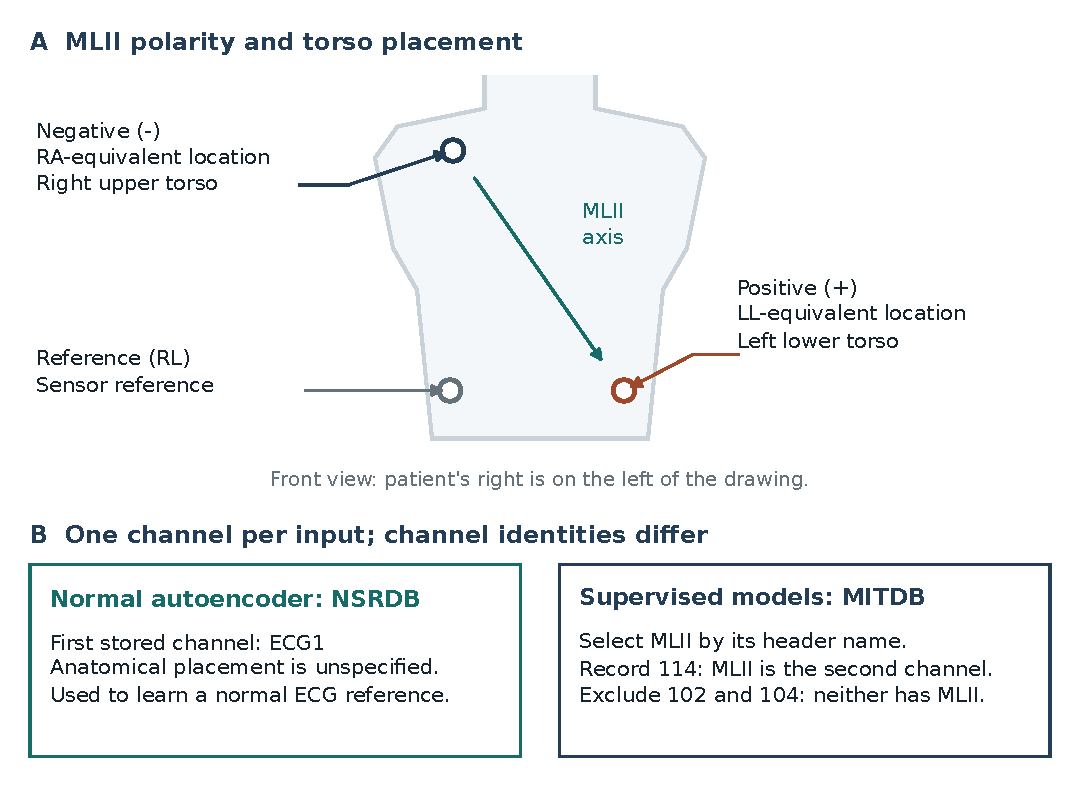
\includegraphics[width=.98\textwidth]{pic/generated/real_lead_positions.pdf}
\caption[MLII polarity and the channel used by each model.]{MLII polarity and
the channel used by each model. Panel A is an anterior-view schematic of the
modified Lead-II axis, with the project's reference connection shown separately;
it is not an exact map of the database electrode coordinates
\cite{physionetLeadFAQ}. Panel B distinguishes the NSRDB ECG1 normal reference
from the MLII input used by the supervised models.}
\label{fig:data-lead-positions}
\end{figure}

\textbf{Reference labels.}
MITDB expert annotations are mapped to the six project outputs as shown in
Table~\ref{tab:data-label-map}. AFib is determined from the rhythm annotation
around a beat; the other targets mainly use beat symbols.

\begin{table}[H]
\centering
\small
\caption{Mapping from MITDB expert annotations to project outputs.}
\label{tab:data-label-map}
\begin{tabular}{lll}
\toprule
Output & MITDB evidence & Interpretation\\
\midrule
N & N, e, j outside AFib/AFL & normal-like/escape group\\
PVC & V, E & ventricular premature or escape beat\\
PAC & A, a, J, S & supraventricular premature beat\\
LBBB & L & left bundle branch block beat\\
RBBB & R & right bundle branch block beat\\
AFib & normal-like beat inside AFIB/AFL rhythm & atrial fibrillation/flutter context\\
\bottomrule
\end{tabular}
\end{table}

The class codes are project groupings, not exact clinical diagnoses or the
standard AAMI five-class scheme. N includes atrial and junctional escape beats;
PVC includes ventricular escape beats; PAC includes nodal and supraventricular
premature beats. AFib combines fibrillation and flutter rhythm annotations
only when the beat symbol maps to N. Other supported beat types retain their
morphology label during AFIB/AFL. Consequently, AFib recall here is neither
pure AF sensitivity nor episode-level AF detection.

Unsupported symbols remain abnormal in binary evaluation and are excluded
from six-class scoring. At runtime, a gated unsupported abnormality still
receives one of the five available subtype labels. The prepared MLII dataset contains 104,755 accepted beats: 63,073
in group N and 41,682 abnormal. Of these, 100,072 have a supported six-class label.

\subsection{Signal cleaning and window construction}

Data preparation converts the two ECG sources into a common input shape: one four-second signal with 512 samples. The supervised preparation rules were fixed for the rerun and are also used
during session prediction. NSRDB retains its original preparation procedure.
Figure~\ref{fig:data-cleaning-real} shows the full transformation for one
healthy NSRDB segment and one MITDB MLII beat.

\subsubsection{Cleaning checks}

Table~\ref{tab:data-cleaning-checklist} lists the preparation steps and their
purpose. Rejected windows do not enter model fitting or evaluation.

\begin{table}[H]
\centering
\small
\caption{Cleaning checklist applied before a signal can become a model input.}
\label{tab:data-cleaning-checklist}
\begin{tabular}{>{\raggedright\arraybackslash}p{2.6cm}>{\raggedright\arraybackslash}p{5.0cm}>{\raggedright\arraybackslash}p{4.3cm}}
\toprule
Step & What is done & Why it matters\\
\midrule
Required channel & NSRDB must provide ECG1; MITDB must provide MLII. Missing
required signals stop processing. & Prevents accidental use of ECG2, V5, V2, or
another non-matching lead.\\
\addlinespace
Sampling rate & NSRDB remains at 128 Hz. MITDB MLII is resampled from 360 Hz to
128 Hz with polyphase anti-aliasing. & Makes every four-second model window
exactly 512 samples.\\
\addlinespace
Band-pass filter & A Butterworth band-pass with prototype order four
and cutoffs 0.5--50 Hz uses forward--backward filtering. For supervised inputs
this is applied within the four-second window \cite{butterworth1930filter,virtanen2020scipy}. & Reduces baseline drift and high-frequency noise while avoiding filter-induced
phase delay.\\
\addlinespace
Amplitude standardisation & Each supervised MLII window is converted to approximately zero mean
and unit standard deviation; NSRDB retains its archived scaling. & Reduces gain differences while preserving the
relative P--QRS--T shape.\\
\addlinespace
Window quality check & Corrected supervised windows must be finite and
non-flat. Both neighbouring R peaks must be observed. & Rejects unusable
inputs. These checks do not establish clinical signal quality or remove all
motion artifacts.\\
\bottomrule
\end{tabular}
\end{table}

\subsubsection{Window construction}

The autoencoder and supervised hierarchy build windows in different ways, but
the final array shape is the same. The autoencoder receives consecutive,
non-overlapping four-second windows from the first stored NSRDB channel. The
supervised MLII windows are aligned to a beat: 200 samples before the R peak
and 312 samples starting at the R peak. During offline experiments, expert annotations give
the R-peak location for alignment and later scoring. During live use, detected
R peaks replace those annotations.

For samples $x_1,\ldots,x_n$ inside one prepared model window, amplitude
standardisation is
\begin{equation}
 z_i=\frac{x_i-\mu}{\sigma+10^{-8}},\qquad
 \mu=\frac{1}{n}\sum_{i=1}^{n}x_i.
\end{equation}
The corrected supervised pipeline filters each extracted window and applies
this operation locally. The original experiment instead standardised each
complete MITDB record before extracting windows. That used test-region signal
statistics during preparation and differed from sensor chunks. The results reported here use the local
preparation procedure. NSRDB remains the frozen
reference checkpoint with its archived input scaling. The real-data audit in
Section~\ref{sec:method-real-case} shows that an archived NSRDB window is not
unit variance; the current cache-building code must not be treated as proof
of the older cache's normalisation.

\subsubsection{Cleaning yield}

The healthy NSRDB recordings produce many candidate windows because complete
records are used instead of short excerpts. Across the 18 complete NSRDB
records, 393,744 candidate windows were formed. The quality checks kept 345,850
windows and rejected 47,894. These accepted windows were then split into
288,673 autoencoder fitting windows and 57,177 validation windows.

MITDB cleaning produces beat-aligned MLII examples. The prepared MLII dataset
contains 104,755 beats: 63,073 in group N and 41,682 abnormal. Unsupported abnormal
symbols are still used for binary abnormality evaluation, but they are excluded
from six-class subtype scoring.

\subsubsection{Preparation during prediction}

The corrected hierarchy applies the same local window filtering,
standardisation and feature order during fitting, offline scoring and
installed use. Database replay first resamples the signal. Sensor acquisition
supplies 128 Hz samples. Labels never enter a prediction.
The live backend waits until there is enough signal around a detected R peak
and enough RR context. It then feeds one prepared MLII window to the frozen
system. Neither supervised model is retrained during prediction.

\begin{figure}[H]
\centering
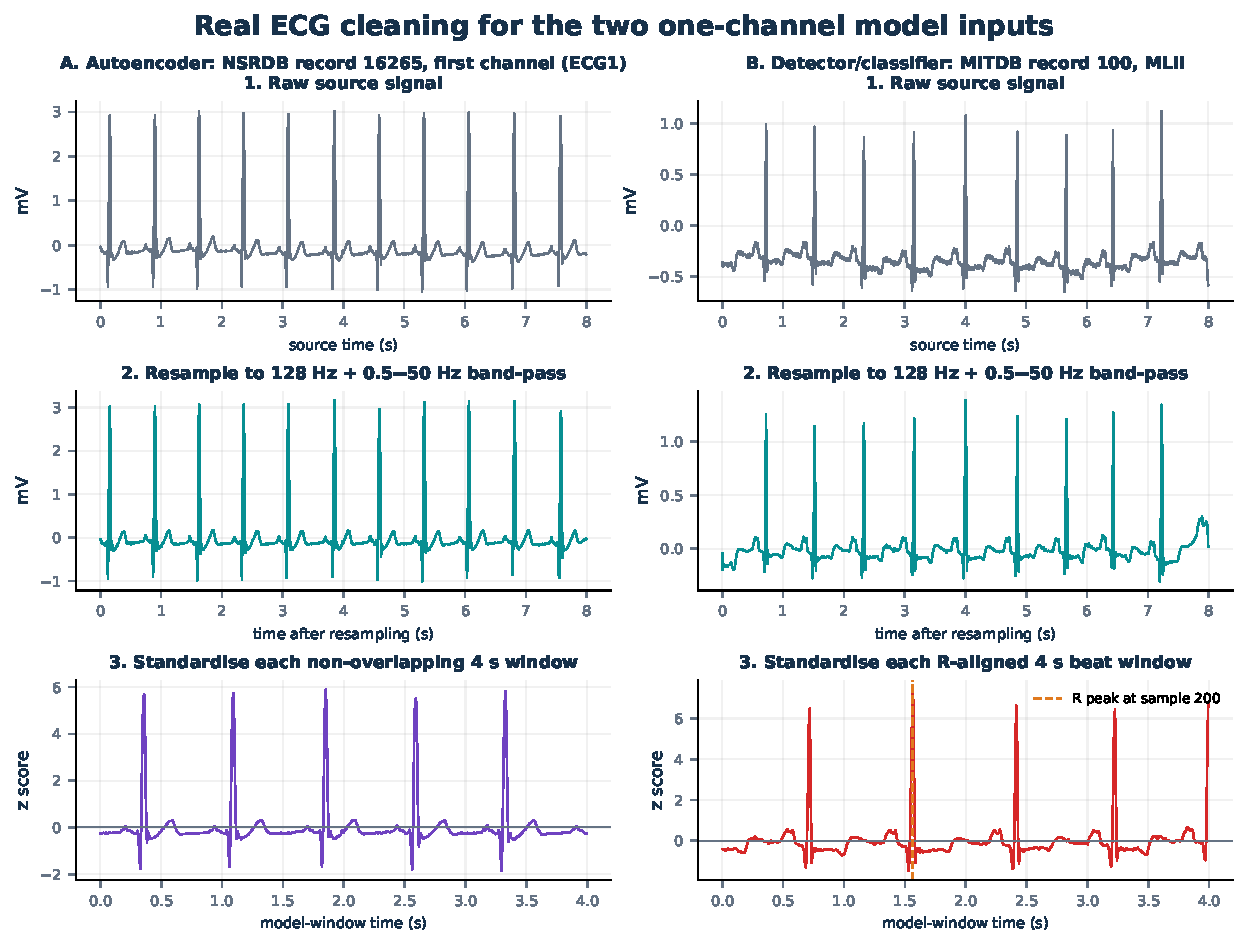
\includegraphics[width=.96\textwidth]{pic/generated/real_data_cleaning_pipeline.pdf}
\caption{Cleaning real ECG for the two roles. The normal-reference example is
the first four seconds of NSRDB 16272/ECG1, with its actual archived scaling.
The supervised example is an MLII beat from MITDB 100, filtered and
standardised within its own window. Both become one 512-sample input;
their channel identities remain different.}
\label{fig:data-cleaning-real}
\end{figure}

\subsection{Model inputs and data allocation}

Data preparation decides which cleaned examples are allowed to fit a model,
which examples choose model settings, and which examples are held back for the
final temporal result. Figure~\ref{fig:data-feed-real} shows this flow from
raw source to frozen prediction.

\subsubsection{Prepared inputs}

After cleaning, the study keeps two kinds of prepared object:
\begin{itemize}
    \item \textbf{NSRDB window:} a normal-reference $[1,512]$ window from the first
    stored ECG channel. It has no arrhythmia label and is used only by the
    normal autoencoder.
    \item \textbf{MITDB beat:} an R-aligned MLII $[1,512]$ window with record
    identity, binary normal/abnormal truth, supported subtype truth when
    available, and RR timing context.
\end{itemize}

The autoencoder input tensor has shape $[B,1,512]$. The supervised detector and
subtype classifier do not receive raw samples alone. Each MITDB beat is
converted into the same 242-value MLII feature vector:
\[
\begin{aligned}
242\ \text{values}={}&230\ \text{morphology, spectrum, statistics, and base-RR values}\\
&+8\ \text{causal RR-history values}\\
&+4\ \text{autoencoder residual values}.
\end{aligned}
\]
The subtype model is fitted only on the five supported abnormal classes: PVC,
PAC, LBBB, RBBB, and AFib.

\subsubsection{Splits}

The autoencoder split is subject-disjoint. A seeded split assigns 15 complete
NSRDB records to fitting and three different records (16420, 16483, and 16795)
to validation. This produces 288,673 fitting windows and 57,177 validation
windows. Validation selects the checkpoint and estimates the normal residual
threshold. There is no separate healthy test because the autoencoder is frozen
before it contributes residual features to MITDB evaluation.

The MITDB split is chronological inside every eligible record:
\begin{itemize}
    \item the first 64\% fits candidate supervised models;
    \item the next 16\% selects the model structures and abnormal-score
    threshold;
    \item a 16-beat gap is removed before both the validation and test
    boundaries during selection; and
    \item the final 20\% evaluates the completed frozen hierarchy.
\end{itemize}
Percentages count accepted beats in chronological order, not exact elapsed
time. Final refitting uses the earlier 80\% while retaining the gap before the test.
The procedure checks that signal windows do not overlap across each boundary. The test had been observed
during earlier development, making this a retrospective known-patient
evaluation with possible optimism.

\subsubsection{Exact model allocation}
\begin{table}[H]
\centering
\small
\caption{Training, validation, and temporal-test data supplied to each model.}
\label{tab:data-model-allocation}
\begin{tabular}{>{\raggedright\arraybackslash}p{2.3cm}>{\raggedright\arraybackslash}p{3.0cm}>{\raggedright\arraybackslash}p{3.0cm}>{\raggedright\arraybackslash}p{3.2cm}}
\toprule
Model & Candidate training & Validation & Final fitting and testing\\
\midrule
Autoencoder & 288,673 first-channel windows from 15 complete NSRDB records & 57,177 windows from 3 different complete NSRDB records & Frozen while every MLII test beat produces four residual features\\
\addlinespace
Abnormality detector & 66,285 MLII beats: 40,469 normal and 25,816 abnormal & 16,029 beats: 9,664 normal and 6,365 abnormal & Fitted on 83,050 development beats; tested on 20,969 temporal-test beats\\
\addlinespace
Subtype classifier & 22,844 supported abnormal MLII beats & 5,651 supported abnormal beats & Fitted on 28,758 supported abnormal beats; conditionally tested on 7,958 supported abnormal beats\\
\bottomrule
\end{tabular}
\end{table}

The supported six-output test contains 20,043 beats: 12,085 N, 1,527 PVC,
589 PAC, 1,481 LBBB, 1,383 RBBB, and 2,978 AFib. Another 926 unsupported
abnormal beats remain in binary testing but not six-class scoring.

\begin{figure}[H]
\centering
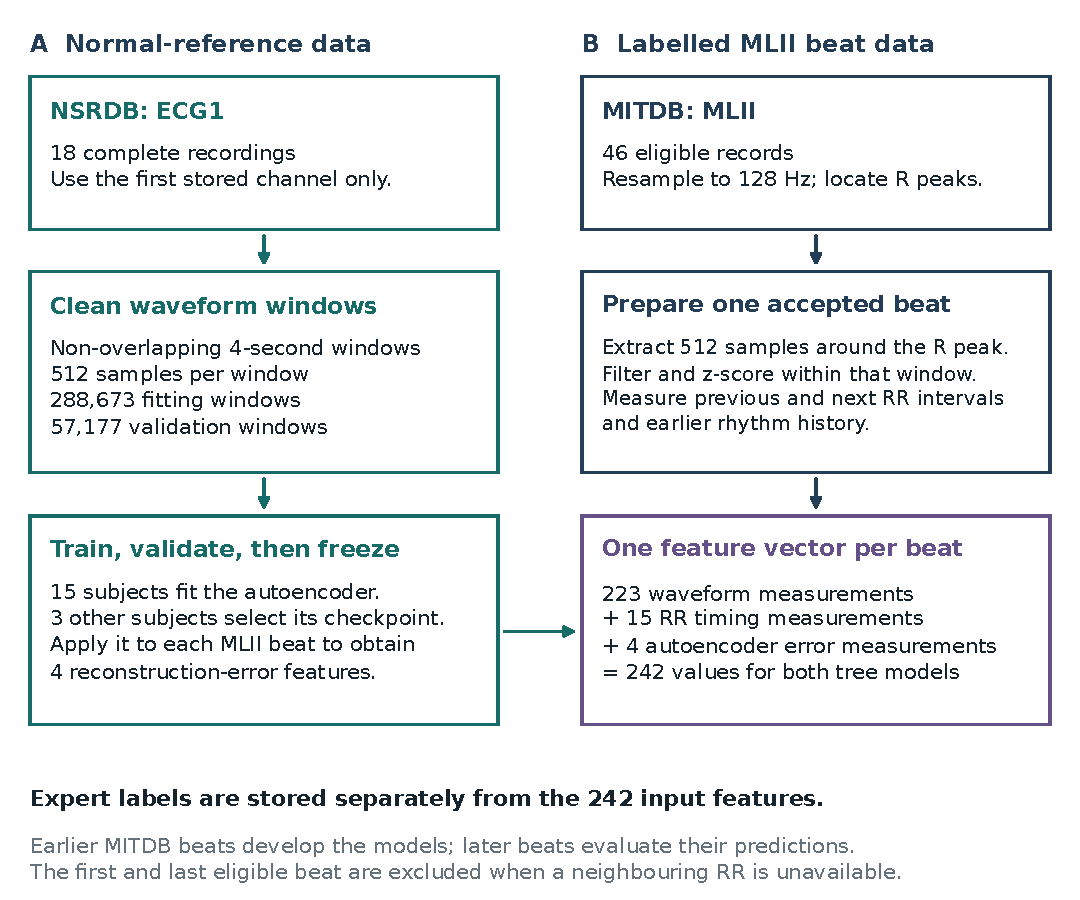
\includegraphics[width=.95\textwidth]{pic/generated/real_data_preparation_flow.pdf}
\caption[Preparation of normal-reference windows and labelled MLII beats.]{Preparation
of normal-reference windows and labelled MLII beats. Panel A develops the frozen
autoencoder from subject-disjoint NSRDB fitting and validation data. Panel B
uses local filtering and standardisation for each MITDB beat, then combines
waveform, RR timing, and frozen-autoencoder residual features. Expert labels
remain separate from the model input.}
\label{fig:data-feed-real}
\end{figure}

\subsubsection{Inputs to the frozen system}

During autoencoder fitting, Gaussian noise with standard deviation 0.03 is
added to each input while the clean NSRDB window remains the target. During
supervised fitting, record-and-class weights reduce domination by long records
and common classes. During prediction, one MLII window, its observed previous and next RR
intervals, and its recent RR history are converted into the same 242-value vector used in the temporal
experiment. A decision of N ends classification for that beat. An abnormal decision passes
the same vector to the subtype model. Section~\ref{ch:theory} explains the theoretical basis of these features and
the two-stage decision. The allocation is evaluated under the protocol in
Section~\ref{ch:method}.

\section{Theoretical foundations}\label{ch:theory}

This section explains the theoretical basis of the ECG system. The system combines
MLII waveform shape, RR timing, and autoencoder residuals in two supervised
Extra Trees ensembles. These components provide complementary information
about beat shape and rhythm.

The explanation follows one beat from measured voltage to the final label.
The equations define the main operations and explain how they contribute to
classification. The three trained components
are a normal-reference autoencoder, a normal-versus-abnormal tree ensemble, and
an abnormal-subtype tree ensemble. The autoencoder learns by changing neural
weights to lower reconstruction error; the tree ensembles learn by choosing
weighted, entropy-reducing splits. These are different forms of training.

\subsection{Why ECG evidence has more than one form}

An ECG is a voltage signal over time. For arrhythmia classification, useful
evidence appears at two related scales. The first is beat-scale morphology:
what the P--QRS--T shape looks like around one R peak. The second is rhythm
timing: when the beat occurs relative to neighbouring beats. The final model
uses both because they answer different questions.

\begin{figure}[H]
\centering
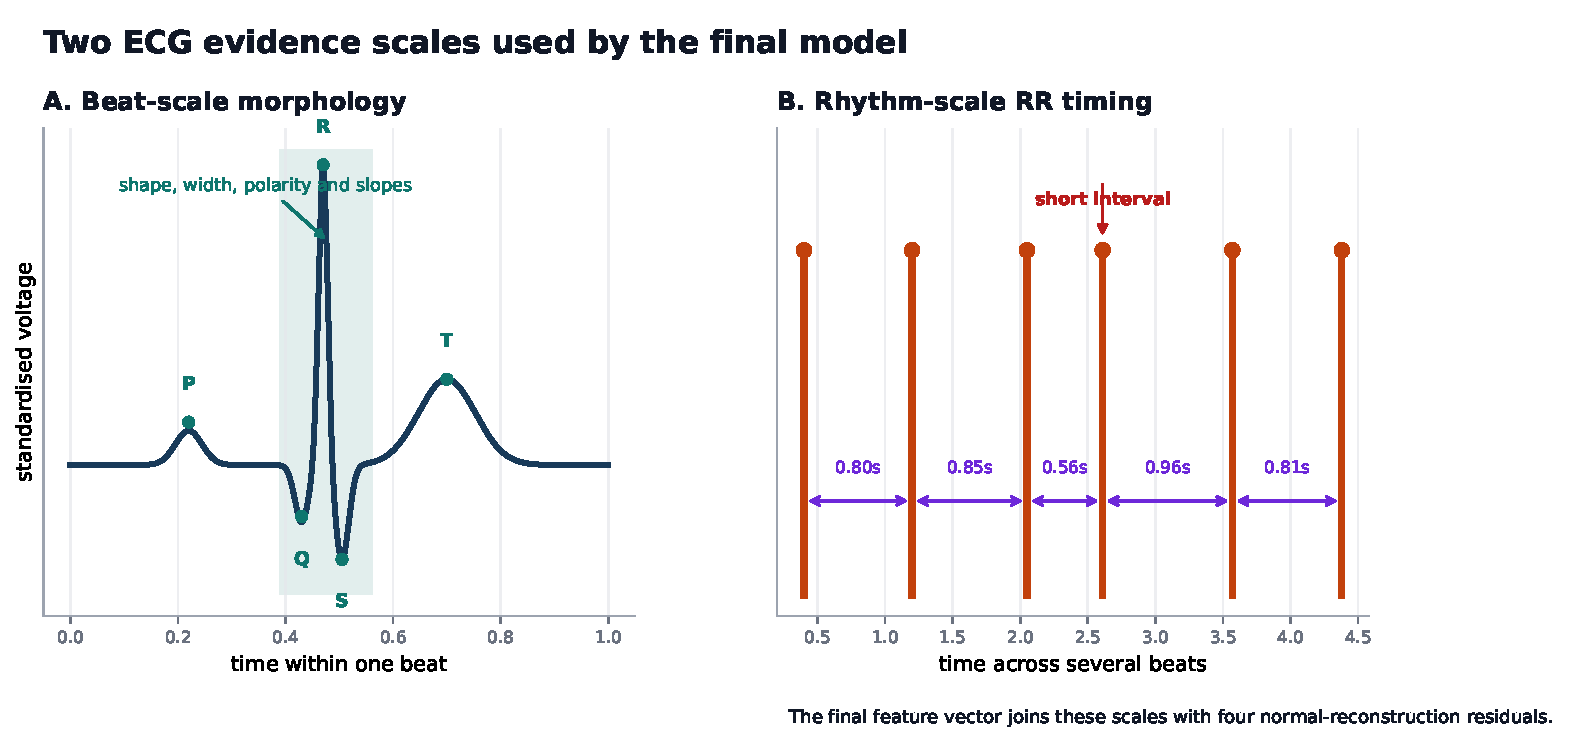
\includegraphics[width=.98\textwidth]{pic/generated/theory_evidence_scales.pdf}
\caption{Two evidence scales used by the final model. Morphology describes the
local shape of a beat; RR timing describes rhythm context around the beat.}
\label{fig:theory-evidence-scales}
\end{figure}

PVC, LBBB, and RBBB can strongly affect QRS shape, width, slopes, and polarity.
PAC and AFib may be easier to detect when timing evidence is also present:
premature beats create short RR intervals, pauses create long RR intervals, and
AFib creates repeated irregularity. Published heartbeat-classification work
also shows the value of combining waveform morphology with heartbeat-interval
features \cite{dechazal2004heartbeat,mousavi2019seq2seq}.

\begin{figure}[H]
\centering
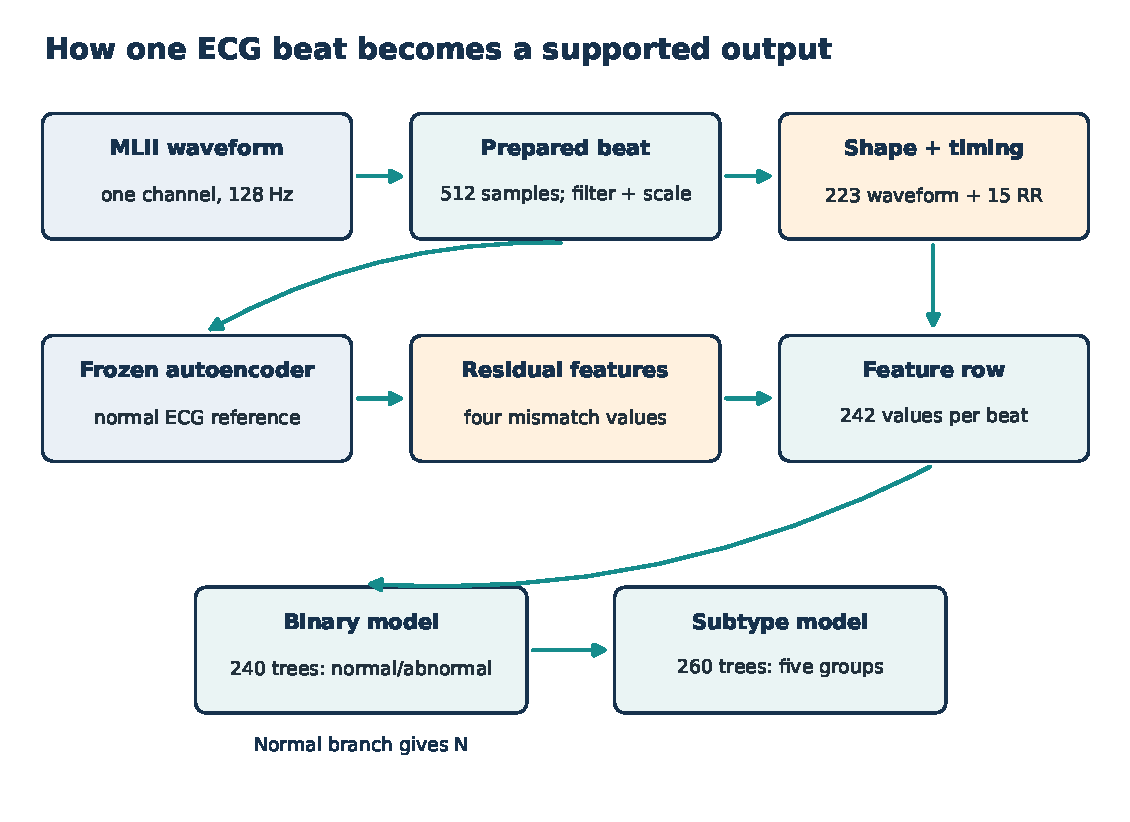
\includegraphics[width=.98\textwidth]{pic/generated/theory_learning_map.pdf}
\caption[Learning map for the final ECG system.]{Reading map for the final system. ECG signal preparation produces one
512-sample window. Three complementary feature groups make one 242-value row.
The frozen autoencoder creates residual features; the two fitted tree
ensembles make the final decision. Labels are used during supervised fitting,
never as input features at prediction time.}
\label{fig:theory-learning-map}
\end{figure}

\subsection{From voltage to a comparable four-second window}

An electrode channel measures a sequence of voltage differences. Sampling at
128 samples per second turns four seconds into $T=4(128)=512$ numbers. The
MITDB waveform is originally sampled at 360~Hz and is resampled to 128~Hz
before beat extraction. Anti-aliasing in the resampling step prevents
high-frequency content from appearing falsely at lower frequencies. The
normal-reference NSRDB channel is already sampled at 128~Hz. Its header calls
the first channel ECG1; the supervised and installed beat input is MLII.
These channel names should not be treated as interchangeable anatomical lead
names \cite{mitdb,nsrdb}.

For supervised examples, an observed R peak is placed at sample 200. Thus a
window contains 200 samples before and 312 samples from that point onward.
The R peak is a useful alignment anchor because many important morphological
changes occur in or near the QRS complex. The normal-reference autoencoder
instead receives consecutive, non-overlapping four-second windows; it does
not need beat labels or R-peak annotations. Figure~\ref{fig:theory-learning-map}
shows where the two streams meet.

The corrected supervised path applies a Butterworth band-pass filter with prototype order four
and 0.5--50~Hz cutoffs to \emph{each} 512-sample window. Forward--backward
filtering removes the phase shift that a one-directional filter would introduce
at an R peak. The lower cutoff attenuates slowly changing baseline, and the
upper cutoff attenuates faster interference. It does not imply that all noise
or motion artifact has disappeared \cite{butterworth1930filter,virtanen2020scipy}.
The NSRDB preparation filters longer recording blocks before making windows;
its archived windows retain their historical scaling, as audited in
Section~\ref{sec:method-real-case}. The local standardisation equation below
describes the corrected supervised MLII path.

If $u_t$ is the filtered voltage in one window, the model receives
\begin{equation}
 x_t=\frac{u_t-\bar u}{s_u+10^{-8}},\quad
 \bar u=\frac{1}{T}\sum_{t=1}^{T}u_t,\quad
 s_u=\sqrt{\frac{1}{T}\sum_{t=1}^{T}(u_t-\bar u)^2}.
 \label{eq:theory-window-zscore}
\end{equation}
Subtracting the window mean removes a local offset. Dividing by its standard
deviation reduces gain differences between recordings. The waveform keeps its
\emph{relative} shape and timing, but absolute millivolt amplitude is no longer
directly available to the model. Flat or non-finite windows are rejected.
Because scaling is calculated inside the current window, later test signal
statistics are not needed when preparing an earlier training beat.

\subsection{Feature extraction theory}

The raw 512-sample MLII window contains more detail than the final tree models
need. Small changes in R-peak alignment or noise can change many raw sample
values. The system therefore converts the window into compact measurements
that keep useful ECG evidence while reducing unnecessary sample-level detail.

\begin{figure}[H]
\centering
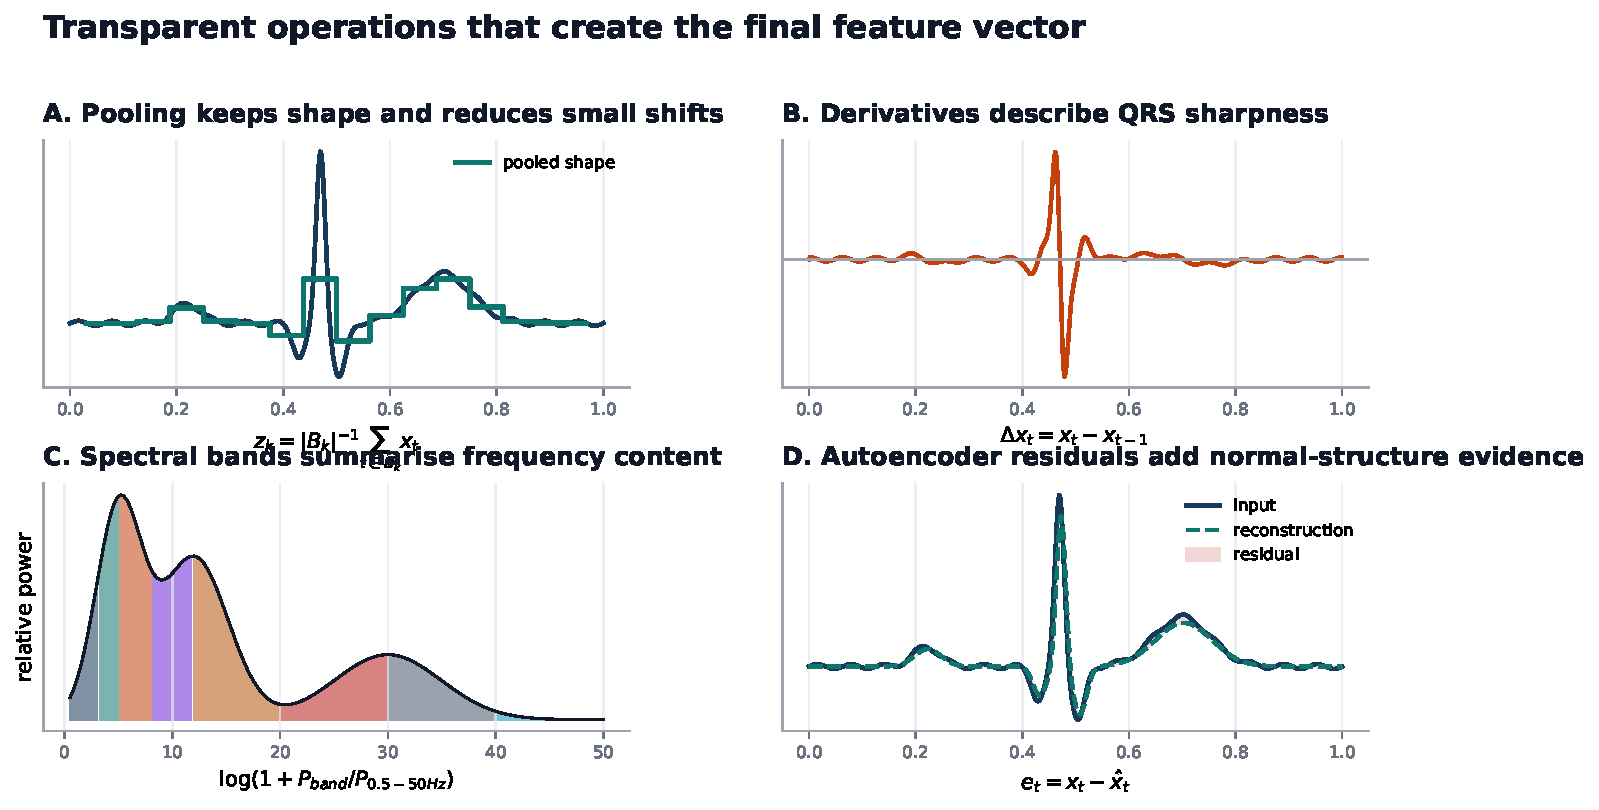
\includegraphics[width=.98\textwidth]{pic/generated/theory_feature_math.pdf}
\caption{Feature-extraction operations behind the final 242-value vector. The
tree models learn from compact numerical evidence, not from raw ECG samples
directly.}
\label{fig:theory-feature-math}
\end{figure}

For a pooled region $B_k$, the pooled value is
\begin{equation}
 z_k=\frac{1}{|B_k|}\sum_{t\in B_k}x_t.
\end{equation}
Pooling keeps the average shape in a small region and makes the representation
less sensitive to a one- or two-sample shift. The final system uses 64
whole-window pooled values and 80 central morphology pooled values.

The derivative
\begin{equation}
 \Delta x_t=x_t-x_{t-1}
\end{equation}
describes how quickly voltage changes. This matters because QRS abnormalities
often change slopes and sharpness. The system keeps 60 pooled derivative values
from the central beat region.

Frequency features describe how signal energy is spread from 0.5 to 50~Hz. For
a frequency band $b$, the relative band feature is
\begin{equation}
 s_b=\log\left(1+\frac{P_b}{P_{0.5-50}}\right),
\end{equation}
where $P_b$ is the power inside the band and $P_{0.5-50}$ is total power in the
ECG band used by the feature extractor. This band-limited view follows the
general ECG idea of keeping physiological content while reducing drift and
high-frequency interference
\cite{kligfield2007standardization,butterworth1930filter}.

Eleven summary statistics add scale, range, energy, skewness, and kurtosis.
Together, the waveform, derivative, spectral, and statistical values form 223
non-RR, non-autoencoder features.

The spectrum is computed with a discrete Fourier transform. For a 512-sample
window, the transform coefficient at frequency index $k$ is
\begin{equation}
 X_k=\sum_{t=0}^{T-1}x_t\exp\!\left(-\frac{2\pi\mathrm{i}kt}{T}\right),
 \qquad P_k=|X_k|^2.
 \label{eq:theory-dft}
\end{equation}
The implementation sums $P_k$ in eight frequency bands between 0.5 and
50~Hz and divides each sum by total power in that range before applying
$\log(1+\cdot)$. The logarithm reduces differences between the relative-power values. These values describe
the distribution of variation by frequency; they are not separate clinical
diagnoses. The eleven statistics include mean, standard deviation, minimum,
maximum, range, mean absolute value, root-mean-square amplitude, derivative
spread and maximum slope, skewness, and excess kurtosis. Skewness describes
asymmetry and kurtosis describes unusually large deviations. The exact count
is $64+80+60+8+11=223$. This count matches the implemented feature vector.

\subsection{RR timing theory}

Let $r_i$ be the time of the R peak of beat $i$. The RR interval is
\begin{equation}
 RR_i=r_i-r_{i-1}.
\end{equation}
RR values describe rhythm. A short interval can suggest a premature beat. A
long interval can suggest a pause. Repeated interval changes support rhythm
irregularity.

The final live system classifies a beat only after it has enough context to
compute the same RR information used in the final experiment. It uses seven
base RR values, including previous RR, next RR, local mean RR, interval ratios,
local coefficient of variation, and heart rate. It then appends eight
history-based values from already completed intervals: median, interquartile
range, median absolute deviation, RMSSD, pNN50, relative range, trend, and
latest interval change.

RMSSD is one example:
\begin{equation}
 \mathrm{RMSSD}=\sqrt{\frac{1}{K-1}\sum_{j=2}^{K}(RR_j-RR_{j-1})^2}.
\end{equation}
The next-RR requirement is important. It delays the streaming decision until the following peak is observed and
allows the same RR features to be used in offline and live processing.

For clarity, the seven base values are previous RR, next RR, mean of up to ten
earlier intervals, previous/mean, next/mean, interval coefficient of
variation, and heart rate $60/RR_{\mathrm{previous}}$. The eight additional
values summarise up to twenty already completed intervals. The interquartile
range is the 75th minus the 25th percentile; median absolute deviation is
the median distance from the median; and $\mathrm{pNN50}$ is the fraction of
successive interval differences exceeding 0.05 seconds. A trend and latest
relative change capture direction. These quantities provide rhythm context
without giving a class label to the model. ``Next RR'' is available only after
the following R peak is observed, so this system makes a delayed beat decision
rather than an instantaneous R-peak decision.

\subsection{Normal-only reconstruction theory}

An autoencoder contains an encoder $f_\theta$ and decoder $g_\phi$. It is
trained to reconstruct a normal ECG window $x$:
\begin{equation}
 \hat{x}=g_\phi(f_\theta(x)), \qquad
 \min_{\theta,\phi}\frac{1}{T}\sum_{t=1}^{T}(x_t-\hat{x}_t)^2.
 \label{eq:ae-objective}
\end{equation}
This follows the representation-learning idea of autoencoders
\cite{hinton2006autoencoder}. The final autoencoder is trained with a
denoising objective: small Gaussian noise is added to the input while the
target remains the clean normal window. Denoising encourages stable structure
instead of exact noise copying \cite{vincent2008denoising}.

\begin{figure}[H]
\centering
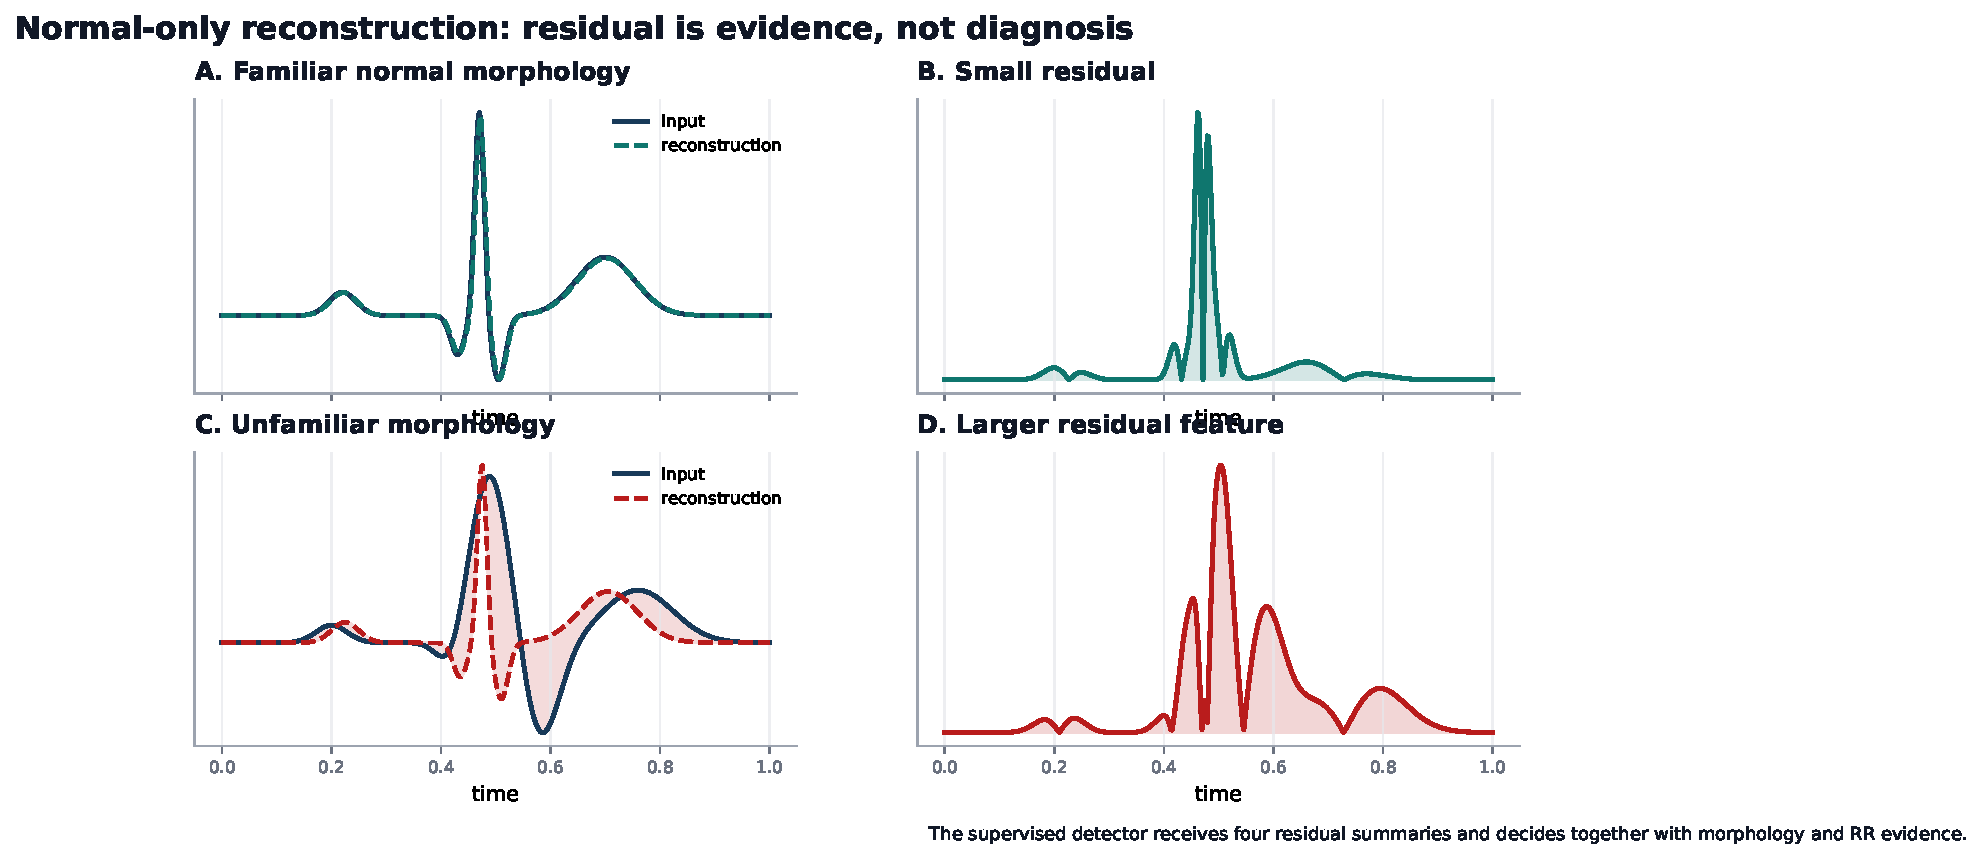
\includegraphics[width=.98\textwidth]{pic/generated/theory_reconstruction_principle.pdf}
\caption{Normal-only reconstruction principle. A larger residual can indicate
novelty, but it is evidence only; the final arrhythmia decision is made by the
supervised hierarchy.}
\label{fig:theory-reconstruction-principle}
\end{figure}

If the autoencoder has learned common normal structure, an unfamiliar or
abnormal beat may be reconstructed less accurately. This is the one-class
anomaly detection idea \cite{chandola2009anomaly}. It is not a guarantee. A
flexible decoder may reconstruct an abnormal waveform well, and noise may
create a large residual for a normal waveform. Therefore, the final system uses
autoencoder mismatch as four supervised input features, not as the final
diagnosis rule.

Let $e_t=x_t-\hat{x}_t$ be the residual. The four residual features are:
\begin{align}
 e_{\mathrm{MAE}} &= \frac{1}{T}\sum_t |e_t|,\\
 e_{\mathrm{MSE}} &= \frac{1}{T}\sum_t e_t^2,\\
 e_{\mathrm{local}} &= \frac{1}{|Q|}\sum_{t\in Q}|e_t|,\\
 e_{\Delta} &= \frac{1}{T-1}\sum_{t=2}^{T}|e_t-e_{t-1}|.
\end{align}
Here $Q$ is the central 240-sample region used by the feature extractor,
defined in Section~\ref{ch:architecture}. The four features measure
whole-window mismatch, squared mismatch, central morphology
mismatch, and residual sharpness. The final architecture appends these four
values to the MLII waveform and RR features.

\subsubsection{What the encoder and decoder actually compute}

The implemented autoencoder is a one-dimensional convolutional network. A
convolution learns a small template and slides it across time. For output
channel $j$ at time $t$, a simplified convolution is
\begin{equation}
 h_{j,t}=b_j+\sum_{c}\sum_{m=0}^{K-1}W_{j,c,m}x_{c,t+m}.
 \label{eq:theory-convolution}
\end{equation}
The learnable numbers $W_{j,c,m}$ and $b_j$ determine which short patterns
activate the channel. A first layer may respond to a steep QRS slope; later
layers can combine such responses over longer time spans. The actual network
uses four encoder blocks to reduce time resolution from 512 to 32 positions
while increasing the channel count to 256. Four decoder blocks restore the
waveform. Figure~\ref{fig:final-ae-layers} gives the verified tensor sizes.

Several architectural functions have distinct purposes. Group normalisation
stabilises intermediate activations. LeakyReLU keeps a non-zero slope for
negative activations, which helps gradients propagate. Residual connections
add a block's input to its transformed output, providing a shorter route for
both signal and gradient flow. Dilation rates 1, 2, 4, and 8 widen the
bottleneck's temporal view without proportionally increasing parameters.
Decoder skip connections pass selected encoder detail forward, scaled by
0.5 in this checkpoint; this helps restore ECG shape but also limits direct
copying. Dropout randomly suppresses activations during fitting to discourage
over-reliance on individual pathways. The last layer is linear so it can
produce both positive and negative standardised voltages
\cite{he2016resnet,ronneberger2015unet,srivastava2014dropout}.

\subsubsection{How the autoencoder lowers reconstruction loss}

Let $x^{(i)}$ be a clean normal window and let
$\epsilon^{(i)}_t\sim\mathcal{N}(0,0.03^2)$ be freshly drawn Gaussian noise.
The training input is $\widetilde x^{(i)}=x^{(i)}+\epsilon^{(i)}$, while the
target is still $x^{(i)}$. For a mini-batch $B$ the actual fitting objective is
\begin{equation}
 \mathcal{L}_{B}(\theta,\phi)=
 \frac{1}{|B|T}\sum_{i\in B}\sum_{t=1}^{T}
 \left[x^{(i)}_t-g_{\phi}(f_{\theta}(\widetilde x^{(i)}))_t\right]^2.
 \label{eq:theory-denoising-loss}
\end{equation}
Squaring makes large reconstruction errors count more strongly. The network
must predict clean structure from a slightly perturbed signal, so simply
copying the input noise is a poor solution. For one output sample, the
derivative of squared error with respect to reconstruction is proportional to
$2(\hat x_t-x_t)$: an output above the target is pushed downward and one below
the target is pushed upward. Backpropagation applies the chain rule through
the decoder and encoder to find the effect of every learned weight
\cite{vincent2008denoising}.

The fitting loop repeatedly performs four operations: clear old gradients,
compute reconstructed windows, backpropagate $\mathcal{L}_{B}$, and take one
Adam step. Adam tracks moving averages of gradients and squared gradients;
schematically, the update is
\begin{equation}
 m_k=\beta_1m_{k-1}+(1-\beta_1)g_k,\quad
 v_k=\beta_2v_{k-1}+(1-\beta_2)g_k^2,\quad
 \theta_{k+1}=\theta_k-\eta\frac{\widehat m_k}
 {\sqrt{\widehat v_k}+\varepsilon}.
 \label{eq:theory-adam}
\end{equation}
Here $g_k$ is the mini-batch gradient, $\eta$ is the learning rate, and hats
indicate bias correction. The same operation updates decoder parameters
$\phi$. Thus ``reducing loss'' means changing millions of network weights in
a direction estimated to reduce expected reconstruction error; it does not
mean manually adjusting a threshold \cite{kingma2015adam}.

\begin{figure}[H]
\centering
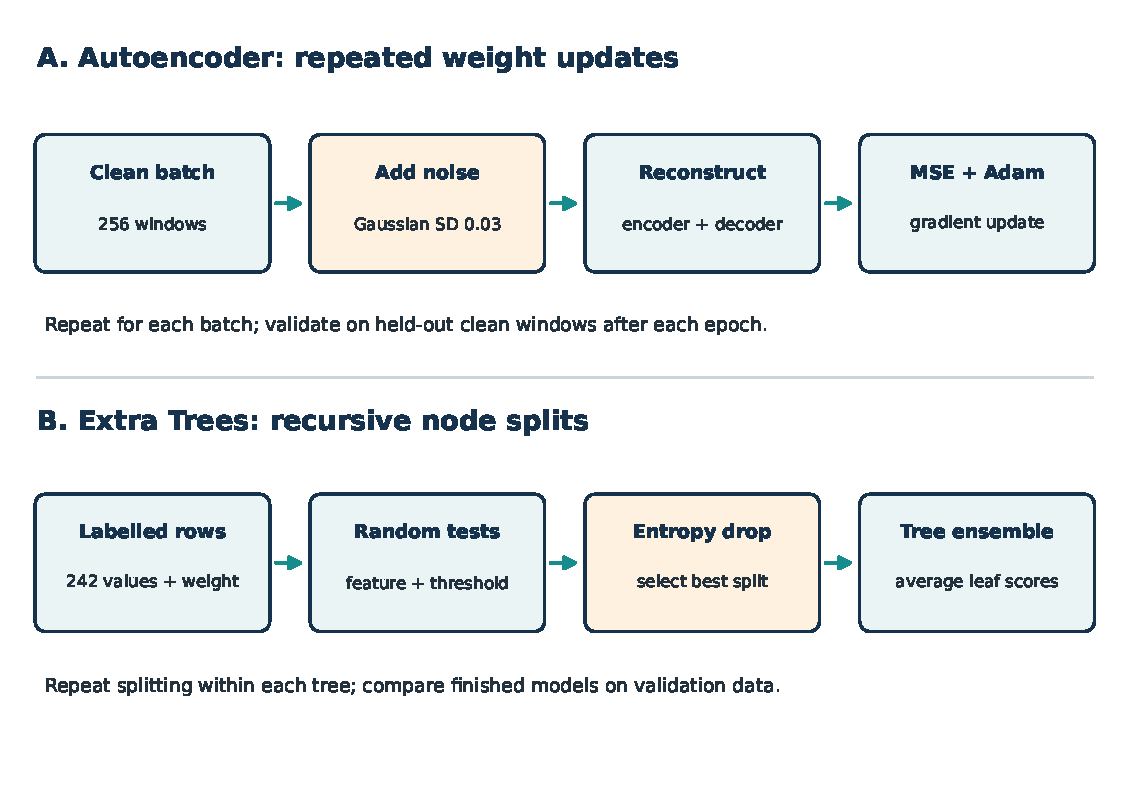
\includegraphics[width=.98\textwidth]{pic/generated/theory_training_mechanisms.pdf}
\caption[Autoencoder and Extra Trees training mechanisms.]{Two distinct learning mechanisms. The autoencoder repeatedly changes
weights from mini-batch reconstruction gradients; an Extra Trees model fixes
each node by comparing randomly proposed splits using weighted entropy. Only
the autoencoder has an epoch-by-epoch reconstruction-loss curve.}
\label{fig:theory-training-mechanisms}
\end{figure}

The implemented training settings and checkpoint-selection rule are specified
in Section~\ref{ch:architecture}. Section~\ref{sec:method-training-inference}
demonstrates the updates numerically and distinguishes the original training
record from the separate real-data teaching demonstration.

\subsection{Hierarchical classification theory}

The hierarchy divides classification into two stages. The first model assigns
a normal or abnormal label. Beats assigned to the abnormal group then enter
the subtype model.

\begin{figure}[H]
\centering
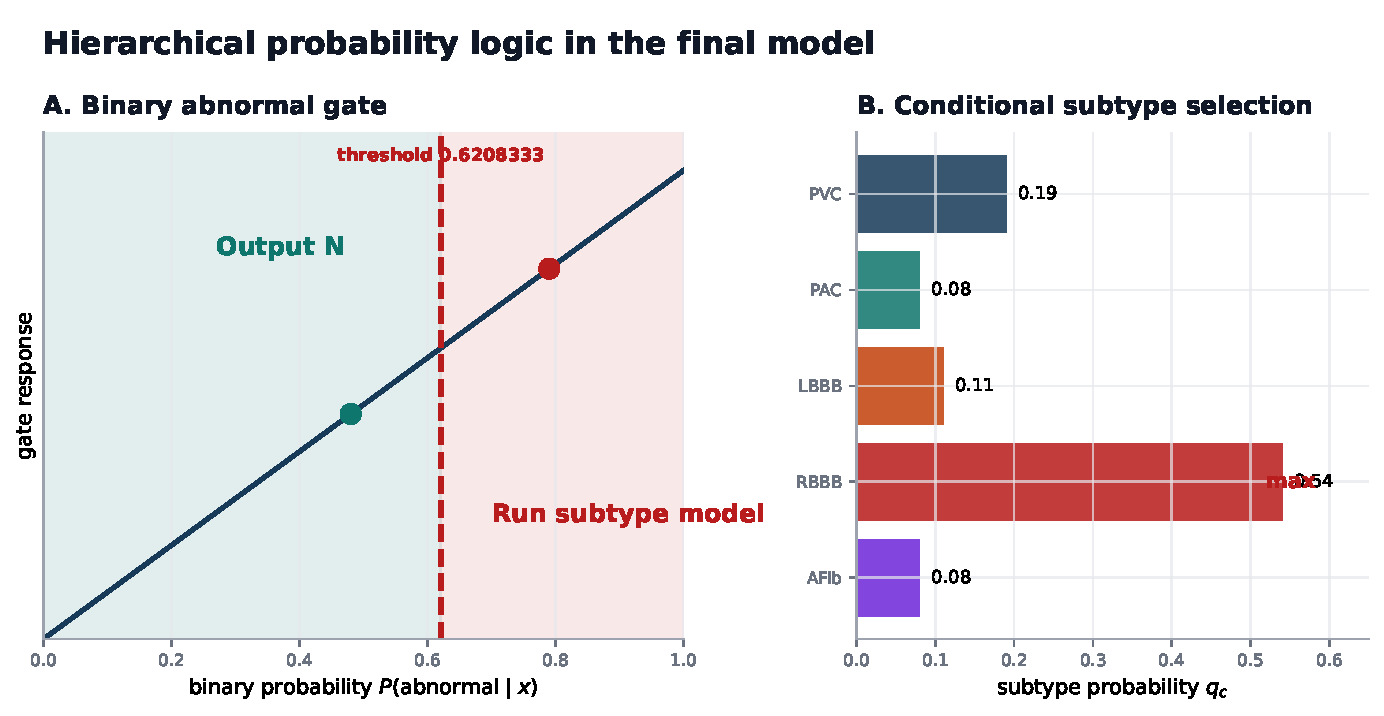
\includegraphics[width=.98\textwidth]{pic/generated/theory_hierarchy_probability.pdf}
\caption{Probability logic of the final hierarchy. The subtype model is
conditional: it is used only after the abnormality gate is passed.}
\label{fig:theory-hierarchy-probability}
\end{figure}

For beat $i$, the binary detector returns an abnormal score $p_i$ from its
242-value feature vector. This score estimates abnormal-class membership
but has not been independently calibrated as a clinical probability.
The final threshold rule is
\begin{equation}
 a_i=\mathbb{1}[p_i>\tau].
\end{equation}
Here $\tau$ is the operating threshold selected using validation data.
If $a_i=0$, the output is N. If $a_i=1$, the subtype model selects the highest
probability among PVC, PAC, LBBB, RBBB, and AFib:
\begin{equation}
 \widehat y_i=\arg\max_{c\in\{1,\ldots,5\}}q_{ic}.
\end{equation}
Here the maximisation already returns an index 1--5. Unsupported abnormal
symbols contribute to binary testing and are excluded from subtype training
and six-class scoring. At inference, every gated beat receives a supported
label. There is no validated unknown-class rejection mechanism.

The tree output is an ensemble score obtained from training-label proportions
in reached leaves. It should not be read as a clinically calibrated disease
probability. In particular, the subtype score $q_{ic}$ is conditional on
taking the abnormal branch; a large $q_{ic}$ does not repair a missed binary
gate. This is why the report evaluates the binary detector, the conditional
subtype model, and the complete six-class decision separately.

\subsection{Why Extra Trees fits this feature design}

The final 242-value vector mixes pooled waveform values, derivatives, spectral
power, signal statistics, RR timing, and autoencoder residuals. Their
relationship to class labels is non-linear. Extra Trees fits this setting by
building many randomised decision trees and averaging their probability
outputs \cite{geurts2006extratrees}.

At a decision-tree node $S$, let $w_i$ be the training weight of beat $i$.
The weighted fraction of class $c$ and its entropy are
\begin{equation}
 p_c(S)=\frac{\sum_{i\in S}w_i\mathbb{1}[y_i=c]}
 {\sum_{i\in S}w_i},\qquad
 H(S)=-\sum_c p_c(S)\log_2 p_c(S),
 \label{eq:theory-weighted-entropy}
\end{equation}
with $0\log_2 0$ defined as zero. Entropy is high when weighted classes are
mixed and zero when a node contains only one class. A proposed split sends
rows to left and right child nodes. Its weighted impurity decrease is
\begin{equation}
 \Delta H=H(S)-\frac{W_L}{W_S}H(S_L)
                 -\frac{W_R}{W_S}H(S_R),
 \qquad W_A=\sum_{i\in A}w_i.
 \label{eq:theory-information-gain}
\end{equation}
For an unweighted toy node with four normal and four abnormal beats, entropy
is one bit. A split putting all normals left and all abnormals right reduces
the two child entropies to zero, giving $\Delta H=1$ bit. Real nodes usually
give a smaller decrease. The tree does not take gradient steps: it selects a
split, partitions the rows, and repeats recursively. Extra Trees randomly
selects candidate features and thresholds at each node, then chooses the
best candidate under this criterion \cite{geurts2006extratrees}.

Each tree ends with leaf nodes. A beat follows feature-threshold questions
from root to leaf, and the leaf's class mixture supplies a score. The ensemble
averages these scores over its trees. Random candidate splits make individual
trees differ; averaging reduces the instability of any one tree. The binary model contains 240 trees and the subtype model contains 260 trees.
Tree count describes ensemble size, whereas an epoch describes one complete
pass through training data in neural-network fitting.

This theory also explains why Extra Trees is suitable for the final data scale.
MITDB contributes many beats but only 45 subject clusters. A very high-capacity
end-to-end neural classifier could learn patient identity instead of robust ECG
rules \cite{zhang2021interpatient}. The Extra Trees hierarchy is still
high-capacity, but it uses transparent tabular evidence and is easier to audit
against the final temporal protocol. This does not mean that tree ensembles are
always better than deep learning.

The binary model learns a normal/abnormal target from all eligible labelled
beats. The subtype model learns only from supported abnormal groups. Both
receive the same feature representation, while the reference labels remain
outside that representation. Section~\ref{sec:method-training-inference}
gives the fitting, weighting, validation, and refitting procedure for each
model. Selection criteria are defined in Section~\ref{ch:method}.

\subsection{Class and patient imbalance theory}

ECG beat datasets are imbalanced in two ways. Some classes are rare, and some
patients contribute many more beats than others. Without weighting, a model can
mostly learn common normal beats or a few large records.

The final training code uses record-aware class weights. For class $c$ in
subject cluster $r$, the weight is proportional to
\begin{equation}
 w_{cr}=\frac{1}{n_c}
 \left(\frac{n_c}{R_c n_{cr}}\right)^\alpha,
 \label{eq:record-weight}
\end{equation}
where $n_c$ is total support for class $c$, $R_c$ is the number of subject clusters
containing class $c$, and $n_{cr}$ is the number of class-$c$ beats in subject cluster
$r$ (records 201 and 202 are combined). Weights are normalised to mean one
and clipped to $[0.05,20]$. The first factor supports class balancing; the second factor reduces
domination by a single record. The exponent $\alpha$ controls how strongly
record balancing is applied and is selected in validation. Class-balanced
learning is important when rare classes would otherwise have little influence
\cite{cui2019classbalanced}.

\subsection{Temporal patient adaptation theory}

ECG morphology contains patient-specific information such as body geometry,
electrode placement, baseline QRS shape, conduction pattern, and background
rhythm. If earlier labelled ECG from a patient is available during development,
the model can adapt to that patient's baseline. This shared patient information can make classification easier than it would
be for a patient whose ECG was absent from development.

This is the theory behind the final temporal-holdout design. It is useful for
monitoring after a labelled calibration period, but it changes the claim. The
final result is a known-patient temporal-continuation result. It should not be
reported as unseen-patient generalisation unless a patient-disjoint experiment
is run. The 16-beat boundary gap reduces direct overlap at the split boundary,
but it does not remove shared patient identity.

\subsubsection{Why training, validation, and testing have different jobs}

Training data changes model parameters: neural weights for the autoencoder,
and split rules and leaf scores for each tree ensemble. Validation data
chooses among checkpoints, tree settings, and the binary operating threshold.
The temporal test then estimates performance after those choices are fixed.
If test labels were used to choose the best threshold, its reported score
would be optimistically biased. In this final rerun, the test did not select
the threshold or candidate, but its labels had been seen during earlier
development. The result is therefore a retrospective known-patient estimate,
not a fresh confirmatory test. Figure~\ref{fig:method-workflow} shows the
chronological allocation and boundary gaps.

\subsection{Validation theory}

Beat-level accuracy alone is not enough. If one patient contributes 2,000
beats, those beats are related. They are not equivalent to 2,000 independent
patients. The final validation therefore reports beat metrics and also uses
subject-clustered uncertainty.

\begin{figure}[H]
\centering
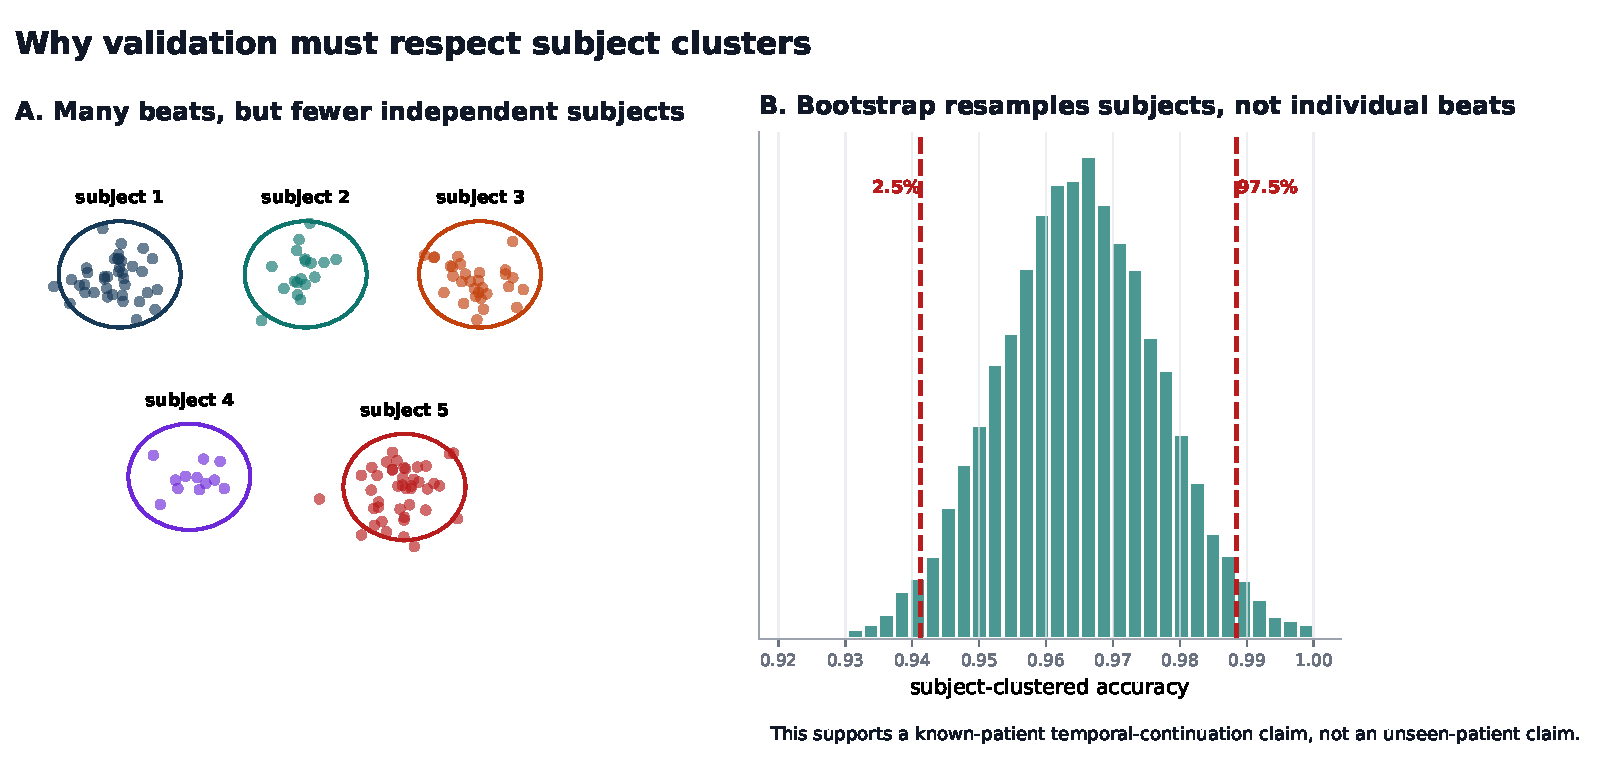
\includegraphics[width=.98\textwidth]{pic/generated/theory_validation_units.pdf}
\caption{Theoretical reason for subject-clustered validation. Clustered
resampling prevents one long record from being treated as many independent
people.}
\label{fig:theory-validation-units}
\end{figure}

Balanced accuracy gives equal weight to class recalls, so normal beats cannot
hide poor abnormal recall. Macro F1 gives each class equal importance, so a
failure on a rare class is visible. Precision--recall style measures are also
important under class imbalance \cite{saito2015pr}. For confidence intervals,
the final experiment resamples complete subject clusters rather than individual
beats, following the general diagnostic-statistics principle that clustered
data need clustered analysis \cite{rutter2000clustered}.

A confusion matrix counts every true/predicted class pair, making aggregate
accuracy easier to interpret. Section~\ref{ch:method} defines the metrics and
bootstrap procedure. Subject-clustered uncertainty does not correct for prior
test exposure or establish generalisation to patients absent from development.

\subsection{Summary of the theoretical framework}

\begin{table}[H]
\centering
\caption{How the theory maps to the implemented final system.}
\label{tab:theory-system-alignment}
\begin{tabular}{>{\raggedright\arraybackslash}p{4.2cm}>{\raggedright\arraybackslash}p{9.0cm}}
\toprule
Theory concept & Implemented in the final system\\
\midrule
Beat-scale morphology & 512-sample MLII window with pooled full-window,
central, and derivative features\\
Rhythm timing & 15 RR features; live scoring waits until next-RR context is
available\\
Normal-only reconstruction & frozen NSRDB autoencoder supplies four residual
features\\
Hierarchical probability & 240-tree binary gate first; 260-tree subtype model
only for gated abnormal beats\\
Class/patient imbalance & record-aware class weighting with validation-selected
record-power parameter\\
Temporal adaptation & earlier MLII timeline trains/selects the model; final
20\% of accepted beats is tested\\
Subject-aware uncertainty & subject-clustered bootstrap over 45 clusters, with
records 201 and 202 treated as one cluster\\
\bottomrule
\end{tabular}
\end{table}

\chapter{Final Model Architecture}\label{ch:architecture}

This chapter explains the final system saved and used by the application. The
installed model is a one-lead MLII beat classifier. It does not use two ECG
leads, does not retrain during live use, and does not make an arrhythmia
decision directly from the autoencoder threshold. The final decision is made by
two supervised Extra Trees models. Both receive the same 242-value feature
vector.

\section{Architecture in one sentence}

For each detected MLII heartbeat, the system takes a 512-sample window aligned
to the R peak, builds waveform, rhythm, and normal-reconstruction features,
sends those features to a binary abnormality gate, and sends only gated
abnormal beats to a five-class subtype classifier.

\begin{figure}[H]
\centering
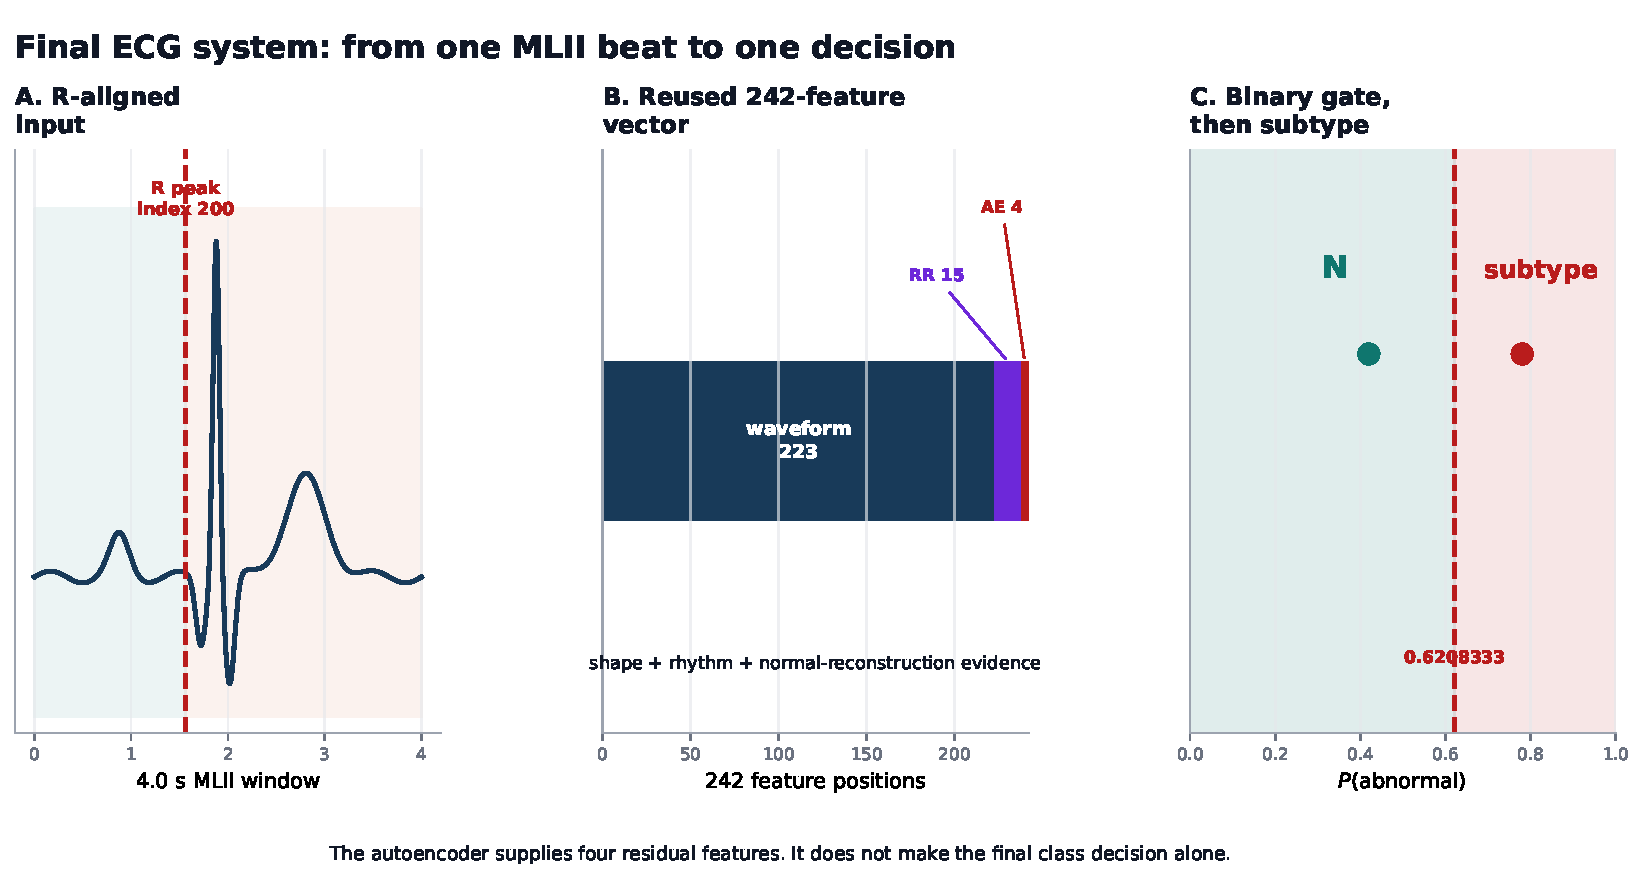
\includegraphics[width=.98\textwidth]{pic/generated/architecture_current_system_flow.pdf}
\caption{Exact runtime order of the final ECG system. The autoencoder supplies
features; the supervised tree models make the final class decision.}
\label{fig:architecture-current-flow}
\end{figure}

\section{Input signal and beat window}

The deployed system accepts one ECG channel. For database replay and final
testing that channel is MIT--BIH MLII, selected by signal name. Records 102 and
104 are excluded because they do not contain MLII. For sensor sessions, the API
requires the user to declare \texttt{lead\_name='MLII'} and rejects other
declared leads. This rule prevents the model from silently scoring a lead that
does not match the supervised training signal.

The classifier is beat based, not arbitrary-window based. The live backend
collects MLII samples, detects R peaks, and waits until enough rhythm context
is available. For a scorable beat, it extracts a fixed 512-sample window at
128 Hz:
\begin{itemize}
\item 200 samples before the R peak;
\item 312 samples after the R peak;
\item total duration of 4.0 seconds.
\end{itemize}
This same window geometry is used in the final temporal-holdout experiment and
in the installed session pipeline.

\begin{figure}[H]
\centering
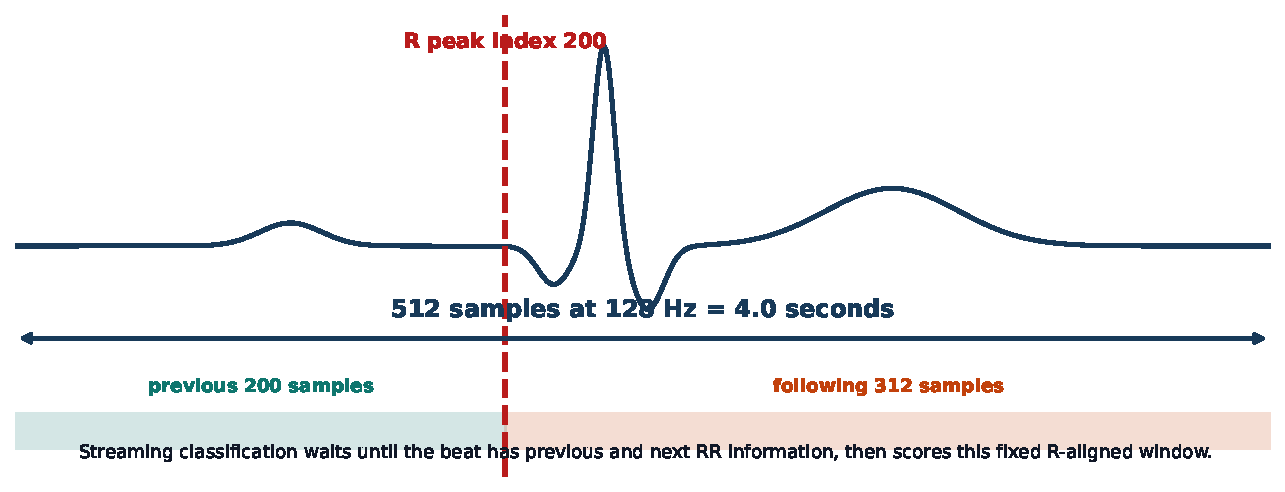
\includegraphics[width=.92\textwidth]{pic/generated/architecture_streaming_window.pdf}
\caption{R-peak-aligned beat window used by the final model. The R peak is at
sample index 200, giving the model pre-QRS context and post-QRS recovery
information.}
\label{fig:architecture-streaming-window}
\end{figure}

\section{Three trained components}

The final system uses three trained components, stored as an autoencoder
checkpoint and a separate hierarchy bundle:
\begin{enumerate}
\item a frozen normal-only autoencoder;
\item a binary Extra Trees abnormality detector;
\item a five-class Extra Trees abnormal-subtype classifier.
\end{enumerate}
The autoencoder is trained first and then frozen. The two supervised tree
models are then fitted on MLII features from the temporal development portion
of MIT--BIH Arrhythmia Database records.

\begin{figure}[H]
\centering
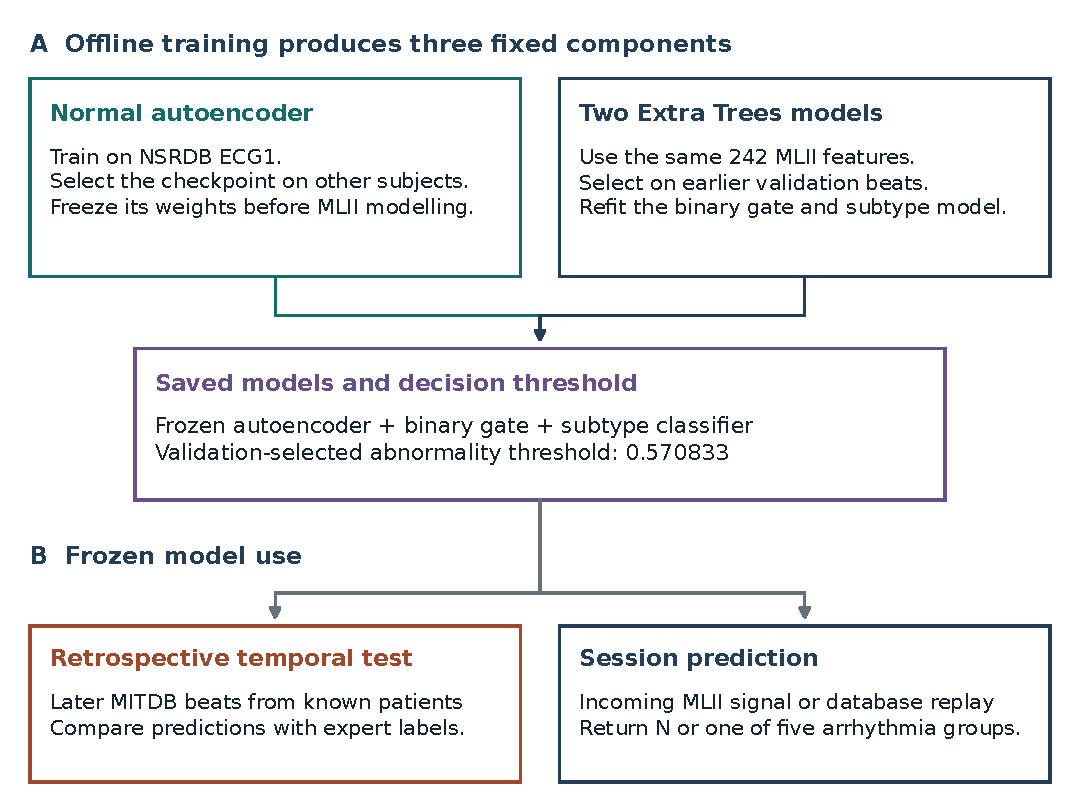
\includegraphics[width=.98\textwidth]{pic/generated/architecture_training_live_map.pdf}
\caption[Training and use of the saved three-component model.]{Training and use
of the saved three-component model. Offline development produces the frozen
autoencoder, binary gate, subtype classifier, and validation-selected threshold.
The same fixed components support retrospective temporal evaluation and session
prediction; session use does not update its parameters.}
\label{fig:architecture-training-live}
\end{figure}

\section{Normal-only autoencoder}

\subsection{Purpose}

The autoencoder is a normal-reconstruction branch. It learns how normal ECG
windows can be reconstructed. The final system then uses reconstruction error
as extra evidence. The autoencoder does not decide ``normal'' or
``arrhythmia'' by itself in the final classifier.

For an input window $x\in\mathbb{R}^{512}$, the autoencoder output is
\begin{equation}
 \widehat x=g_{\phi}(f_{\theta}(x)),
\end{equation}
where $f_{\theta}$ is the encoder and $g_{\phi}$ is the decoder. Training uses
a denoising objective: Gaussian noise with standard deviation 0.03 is added to
the input, but the target remains the clean standardised window. The training
loss is
\begin{equation}
 \mathcal{L}_{AE}=\frac{1}{512}\sum_{t=1}^{512}
 (x_t-\widehat x_t)^2.
 \label{eq:ae-loss-final}
\end{equation}
This objective encourages stable normal morphology instead of copying small
noise patterns \cite{vincent2008denoising}.

\subsection{Network structure}

\begin{figure}[H]
\centering
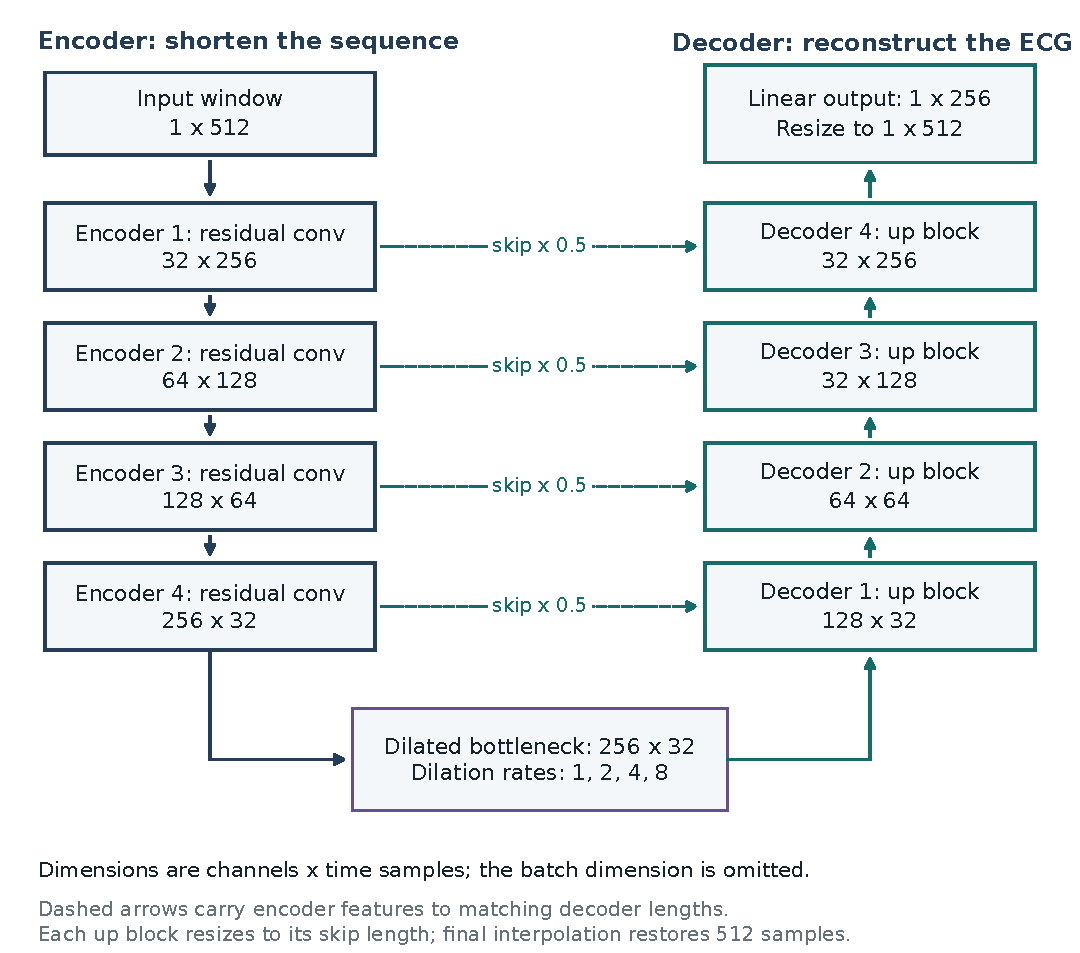
\includegraphics[width=.98\textwidth]{pic/generated/architecture_autoencoder_layers.pdf}
\caption[Autoencoder architecture with verified tensor dimensions.]{Autoencoder
architecture with tensor dimensions verified by a forward pass through the
2,680,641-parameter implementation. Read down the encoder, through the
bottleneck, and up the decoder. Dashed connections concatenate encoder features
scaled by 0.5; decoder outputs match their skip lengths before the final
interpolation restores the 512-sample waveform.}
\label{fig:final-ae-layers}
\end{figure}

Each residual encoder block contains two kernel-seven convolutions, Group
Normalisation, LeakyReLU, dropout, and a residual projection. Four
kernel-three bottleneck blocks use dilation 1, 2, 4, and 8. Dilation increases
the receptive field without deleting time samples. The decoder uses transposed
convolutions and skip connections scaled by 0.5. Each up block resizes its
output to match the corresponding encoder skip. The first up block therefore
returns length 32, the fourth returns length 256, and final linear interpolation
restores length 512. The figure reports these actual tensor dimensions.
The final layer is linear
because the standardised ECG signal contains positive and negative values.

\subsection{Normal-reference data and checkpoint}

The autoencoder checkpoint was developed from complete recordings of all 18
subjects in the MIT--BIH Normal Sinus Rhythm Database. Fifteen subjects supply
288,673 fitting windows and three different subjects supply 57,177 validation
windows. The selected NSRDB header channel is \texttt{ECG1}. The database does
not document this channel as anatomical Lead II, so the report treats it as a
normal ECG reference channel rather than renaming it MLII \cite{nsrdb}.

The final checkpoint uses Adam, learning rate 0.001, batch size 256, and two
epochs. Validation MSE changed from 0.061195 after epoch 1 to the best saved
value, 0.061193, after epoch 2. The autoencoder artifact also stores a
normal-residual threshold of 0.158893, but the final hierarchy does not use
that threshold as the final arrhythmia rule.

\begin{figure}[H]
\centering
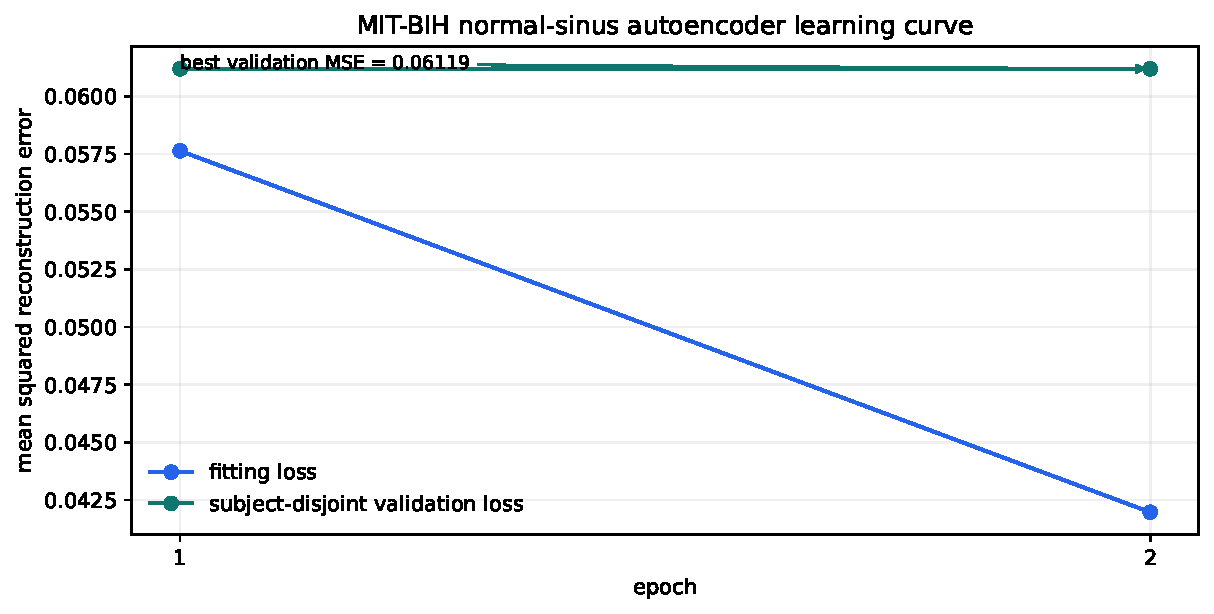
\includegraphics[width=.82\textwidth]{pic/generated/nsrdb_autoencoder_learning_curve.pdf}
\caption[Autoencoder fitting and validation loss.]{Autoencoder fitting and
subject-disjoint validation loss. The checkpoint with the lowest validation
loss is retained before the supervised MLII stages are trained.}
\label{fig:lead-ii-ae-learning}
\end{figure}

\subsection{Four autoencoder residual features}

Let $e_t=x_t-\widehat x_t$ be the reconstruction residual. The final feature
system uses four scalar residual summaries:
\begin{align}
 f_1&=\frac{1}{512}\sum_t|e_t| &&\text{whole-window MAE},\\
 f_2&=\frac{1}{512}\sum_te_t^2 &&\text{whole-window MSE},\\
 f_3&=\frac{1}{240}\sum_{t=104}^{343}|e_t| &&\text{central morphology MAE},\\
 f_4&=\frac{1}{511}\sum_{t=2}^{512}|e_t-e_{t-1}| &&\text{residual-change MAE}.
\end{align}
The central feature focuses on the QRS and nearby morphology. The
residual-change feature becomes large when the reconstruction misses sharp
slopes. These four values are appended to the transparent MLII and RR features.

\begin{figure}[H]
\centering
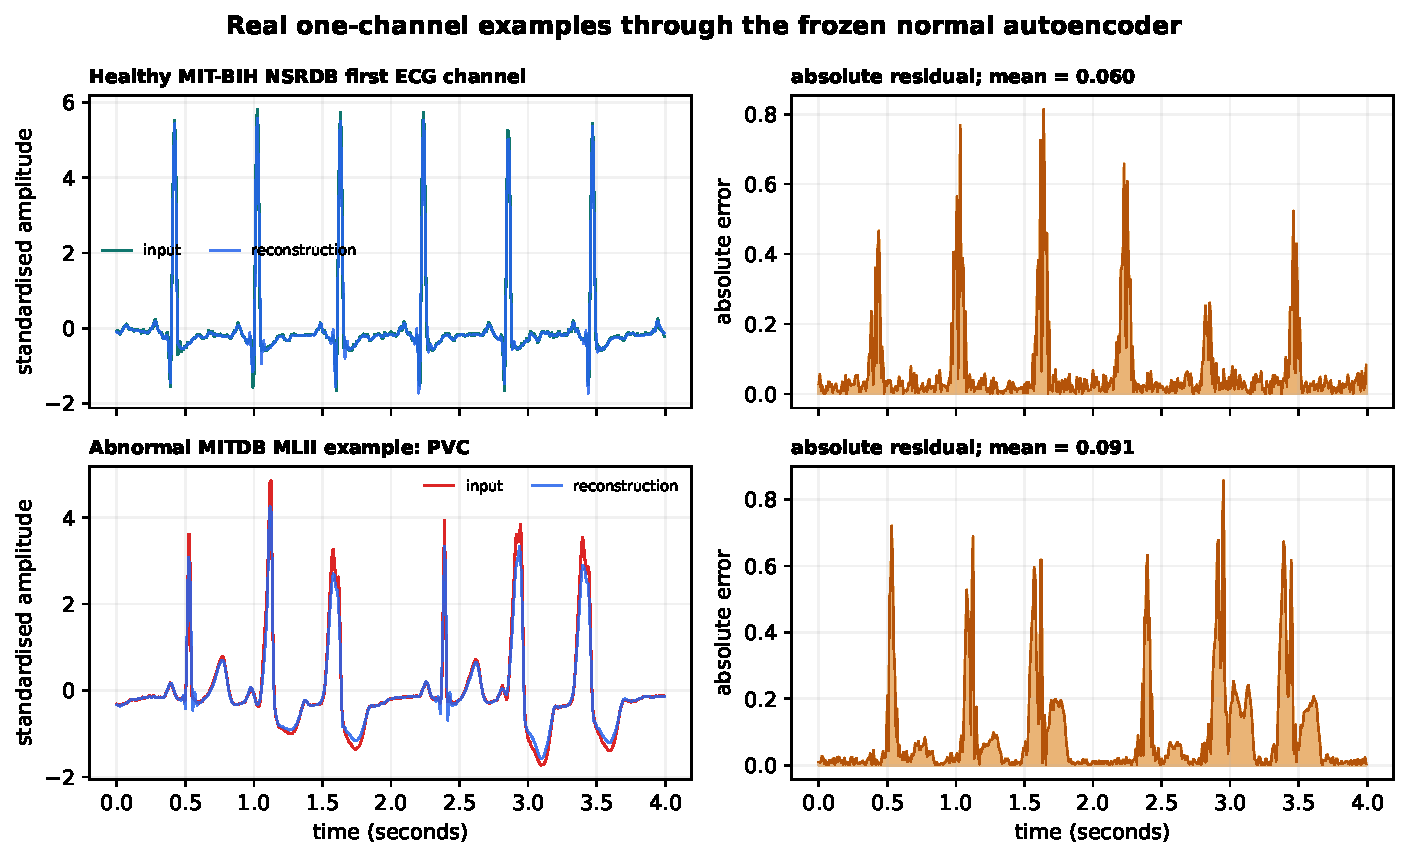
\includegraphics[width=.96\textwidth]{pic/generated/real_autoencoder_processing.pdf}
\caption{Real healthy and abnormal ECG examples through the frozen
autoencoder. The residual between input and reconstruction is converted into
four numerical features for the supervised detector.}
\label{fig:final-real-ae}
\end{figure}

\section{Final 242-value feature vector}

The saved final bundle declares 242 total features, 15 RR features, required
autoencoder features, and four autoencoder residual values. Therefore every
supervised prediction uses:
\begin{equation}
\begin{aligned}
&223\ \text{waveform/spectrum/statistics values}\\
&\quad +15\ \text{RR timing values}\\
&\quad +4\ \text{autoencoder residual values}=242.
\end{aligned}
\end{equation}

\begin{figure}[H]
\centering
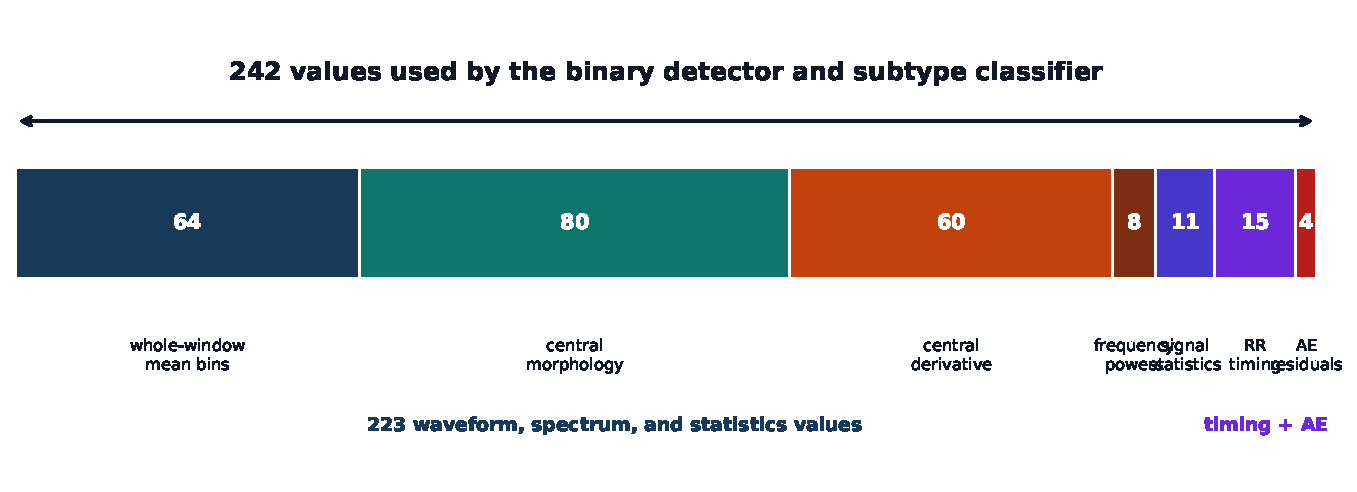
\includegraphics[width=.98\textwidth]{pic/generated/architecture_feature_vector.pdf}
\caption{Feature-vector layout used by both supervised models. The same
242-value vector is passed first to the abnormality detector and, if required,
to the subtype classifier.}
\label{fig:architecture-feature-vector}
\end{figure}

\begin{table}[H]
\centering
\caption{Organised feature groups in the final architecture.}
\label{tab:final-feature-vector}
\begin{tabular}{lrp{8.2cm}}
\toprule
Group & Values & What it tells the model\\
\midrule
Whole-window mean bins & 64 & broad four-second MLII waveform shape\\
Central morphology bins & 80 & P--QRS--T shape around the R peak\\
Central derivative bins & 60 & sharp slopes and rapid QRS changes\\
Frequency-band powers & 8 & relative energy from 0.5 to 50 Hz\\
Signal statistics & 11 & scale, range, energy, skewness, and kurtosis\\
RR timing context & 15 & previous/next interval, local rate, variability,
median, interquartile range, MAD, RMSSD, pNN50, range ratio, trend, and latest
RR change\\
Autoencoder residuals & 4 & how strongly the beat disagrees with the learned
normal-reconstruction pattern\\
\bottomrule
\end{tabular}
\end{table}

The final experiment constructs the same 242 values in two steps: first 230
values are built from 223 MLII waveform/statistical values plus seven base RR
values; then eight causal RR-history values and four autoencoder residual
values are appended. During live/session prediction, the backend builds the
same final vector directly from 223 MLII waveform/statistical values, 15 RR
values, and four autoencoder residual values.

\section{Binary abnormality detector}

The first supervised model is the abnormality detector. It receives all 242
features and estimates $p_i=P(\mathrm{abnormal}\mid x_i)$ for beat $i$. The
selected detector is an Extra Trees classifier with:
\begin{itemize}
\item 240 trees;
\item entropy split criterion;
\item fully grown trees;
\item minimum leaf size of one sample;
\item square-root feature sampling at each split;
\item record/class weighting with record-power $\alpha=0.35$.
\end{itemize}
The decision threshold was selected on the 64--80\% validation region of each
development record:
\begin{equation}
 a_i=\mathbb{1}[p_i>0.5708333].
\end{equation}
If $a_i=0$, the final output is normal class N. No subtype classifier is used
for that beat.

For tree $b$, let $p_b(x_i)$ be the abnormal class proportion in the reached
leaf. The ensemble probability is
\begin{equation}
 p_i=\frac{1}{240}\sum_{b=1}^{240}p_b(x_i).
\end{equation}
Averaging many randomly split trees reduces the instability of one decision
tree while still modelling non-linear links among ECG shape, RR timing, and
autoencoder residuals.

\section{Abnormal-subtype classifier}

The second supervised model is used only after the binary gate marks a beat as
abnormal. It is fitted only on supported abnormal classes 1--5, not on N and
not on unsupported MIT--BIH symbols. The selected subtype model is an Extra
Trees classifier with:
\begin{itemize}
\item 260 trees;
\item entropy split criterion;
\item fully grown trees;
\item minimum leaf size of one sample;
\item one-third feature sampling at each split;
\item record/class weighting with record-power $\alpha=0.25$.
\end{itemize}

For an abnormal beat, the subtype classifier returns probabilities over the
five supported abnormal outputs: PVC, PAC, LBBB, RBBB, and AFib. The final
subtype is
\begin{equation}
 \widehat y_i=\arg\max_{c\in\{1,\ldots,5\}}q_{ic}.
 \label{eq:final-decision}
\end{equation}
The final saved bundle sets \texttt{reject\_low\_confidence=False}. Therefore
the evaluated and installed final pipeline do not add a post-hoc
``Unclassified abnormal'' rejection step; every gated abnormal beat receives
the subtype with the largest subtype probability.

The displayed subtype confidence is conditional on the abnormal branch. It
is an ensemble score, not a calibrated probability of disease. Unsupported
abnormalities can receive an incorrect supported subtype.

\section{Final decision logic}

The complete prediction rule is:
\begin{enumerate}
\item Validate that the input is a 512-sample MLII beat window and that 15 RR
features are available.
\item Reconstruct the same window with the frozen autoencoder.
\item Build the 242-value vector from MLII shape, RR timing, and four
autoencoder residual summaries.
\item Estimate $p_i=P(\mathrm{abnormal}\mid x_i)$ using the 240-tree binary
detector.
\item If $p_i\leq0.5708333$, output N with confidence $1-p_i$.
\item If $p_i>0.5708333$, run the 260-tree subtype model and output the
highest-probability supported subtype.
\end{enumerate}

This is the same hierarchy used in the final temporal-holdout evaluation. The
model does not use test labels while predicting. The labels are used only after
prediction to compute accuracy, F1, confusion matrices, and subject-clustered
uncertainty.

\section{Why this architecture was selected}

\begin{table}[H]
\centering
\caption{Reason for each major final-architecture decision.}
\label{tab:final-design-rationale}
\begin{tabular}{>{\raggedright\arraybackslash}p{3.6cm}>{\raggedright\arraybackslash}p{9.6cm}}
\toprule
Decision & Reason\\
\midrule
MLII-only supervised input & matches the signal available in 46 eligible
MIT--BIH records and avoids hidden two-lead assumptions\\
R-peak alignment & puts comparable cardiac events in comparable positions
inside every 512-sample window\\
Waveform and derivative bins & preserve beat morphology, including sharp QRS
changes\\
Frequency powers and statistics & add compact information about signal energy,
scale, and distribution\\
Fifteen RR features & represent local rate, premature beats, rhythm
irregularity, and recent interval trend using information reproducible during
streaming\\
Normal-only autoencoder & supplies a learned measure of disagreement with
normal ECG structure without requiring arrhythmia labels\\
Two-stage hierarchy & allows unsupported abnormal beats to count in binary
testing without forcing them into one of the five supported subtype labels\\
Extra Trees models & handle mixed feature scales and non-linear interactions
with reproducible tabular-model training\\
Temporal split with gap & evaluates later signal from each record while
removing direct boundary overlap between development and test beats\\
\bottomrule
\end{tabular}
\end{table}

The architecture is therefore best described as a known-patient temporal
continuation system. Its final performance numbers describe later MLII signal
from patients whose earlier MLII signal was available during model development.
They should not be presented as unseen-patient generalisation without a
separate patient-disjoint evaluation.

\section{Experimental design and evaluation}\label{ch:method}

The main experiment evaluated later MLII beats from patients whose earlier
labelled ECG was available during development. Beats were split in
chronological order within each record. This design measures performance on
known patients. The final segment had been viewed during earlier development,
so the reported results form a retrospective evaluation.

\subsection{Evaluation workflow}

Figure~\ref{fig:method-workflow} shows how accepted beats are allocated to
model selection, final refitting, and testing. The normal
autoencoder was already frozen from NSRDB. The supervised experiment then used
only MITDB MLII beats. Candidate models were selected with earlier temporal
regions, refitted before the test boundary, and evaluated only on the final
20\% of accepted beats.

\begin{figure}[H]
\centering
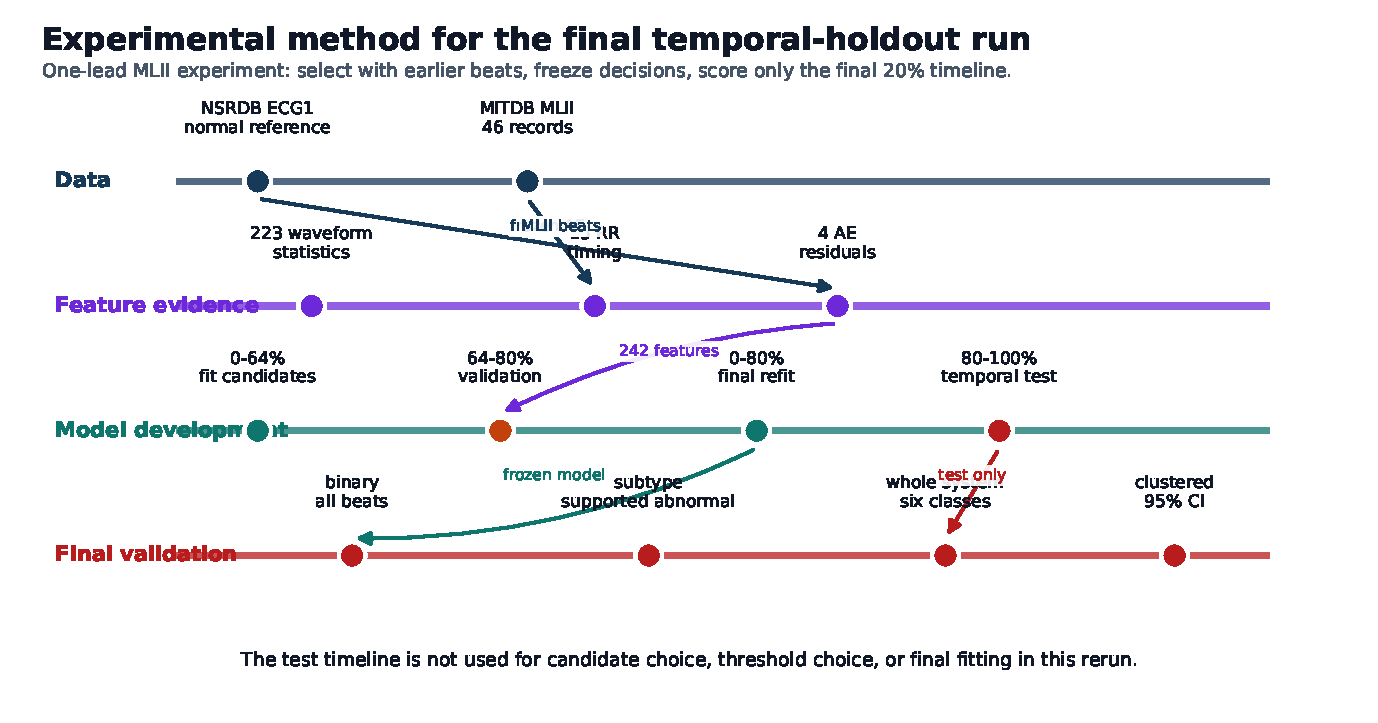
\includegraphics[width=.98\textwidth]{pic/generated/method_final_workflow.pdf}
\caption[Chronological model selection, refitting, and final testing.]{Chronological
selection, refitting, and testing by accepted-beat order. Selection excludes
16 beats before both boundaries; refitting retains only the exclusion before
the test. The test region was observed during earlier development.}
\label{fig:method-workflow}
\end{figure}

\subsection{Research objective and success conditions}

The final experiment asks:
\begin{quote}
After the model has access to the earlier ECG of each patient, how accurately
does it classify that patient's later ECG?
\end{quote}

The primary outcome is whole-system six-class accuracy on the final 20\%
temporal holdout. The planned success conditions were:
\begin{enumerate}
    \item pooled whole-system accuracy above 90\%;
    \item lower bound of the equal-subject 95\% confidence interval above
    90\%; and
    \item total confidence-interval width no greater than three percentage
    points.
\end{enumerate}
The secondary target was recall above 90\% for each supported abnormal
group. Macro F1 and per-class results were also examined because overall
accuracy can hide poor performance on a smaller class.

\subsection{Separation of normal-reference and supervised development}

The data allocation in Section~\ref{ch:data} uses 15 NSRDB subjects for
autoencoder fitting and three separate subjects for checkpoint validation.
The normal-reference checkpoint is frozen before supervised development.
NSRDB windows do not enter the final MITDB temporal test, and MITDB class
labels do not update the autoencoder. The archived NSRDB scaling is retained;
it differs from the beat-local standardisation of supervised MLII windows,
as documented in Section~\ref{sec:method-real-case}.

Both supervised models use the 242-value representation specified in
Section~\ref{ch:architecture}. The fitting equations and numerical examples
are given in Section~\ref{sec:method-training-inference}; the remainder of
this section defines how that procedure was selected and evaluated.

\subsection{Temporal split}

The eligible supervised records are the 46 MITDB records that contain MLII.
Records 102 and 104 were excluded before fitting because their available leads
are V5 and V2, not MLII. Records 201 and 202 are treated as one subject cluster
for uncertainty analysis because they belong to the same person.

Every eligible record is kept in chronological order. Percentages refer to
accepted-beat counts, not exact elapsed recording time. With $n_r$ accepted
beats, the cuts are $\lfloor0.64n_r\rfloor$ and $\lfloor0.80n_r\rfloor$:
\begin{enumerate}
    \item the first 64\% is the candidate-training region;
    \item a 16-beat gap is removed before validation during candidate
    selection;
    \item the 64--80\% region is the validation region;
    \item a 16-beat gap is removed before the final temporal test; and
    \item the final 20\% is the fixed temporal test.
\end{enumerate}
For final fitting, the selected binary and subtype models are refitted on the
earlier 80\% development region after the 16-beat boundary gap before the test
is removed. The test segment itself remains intact.

\begin{figure}[H]
\centering
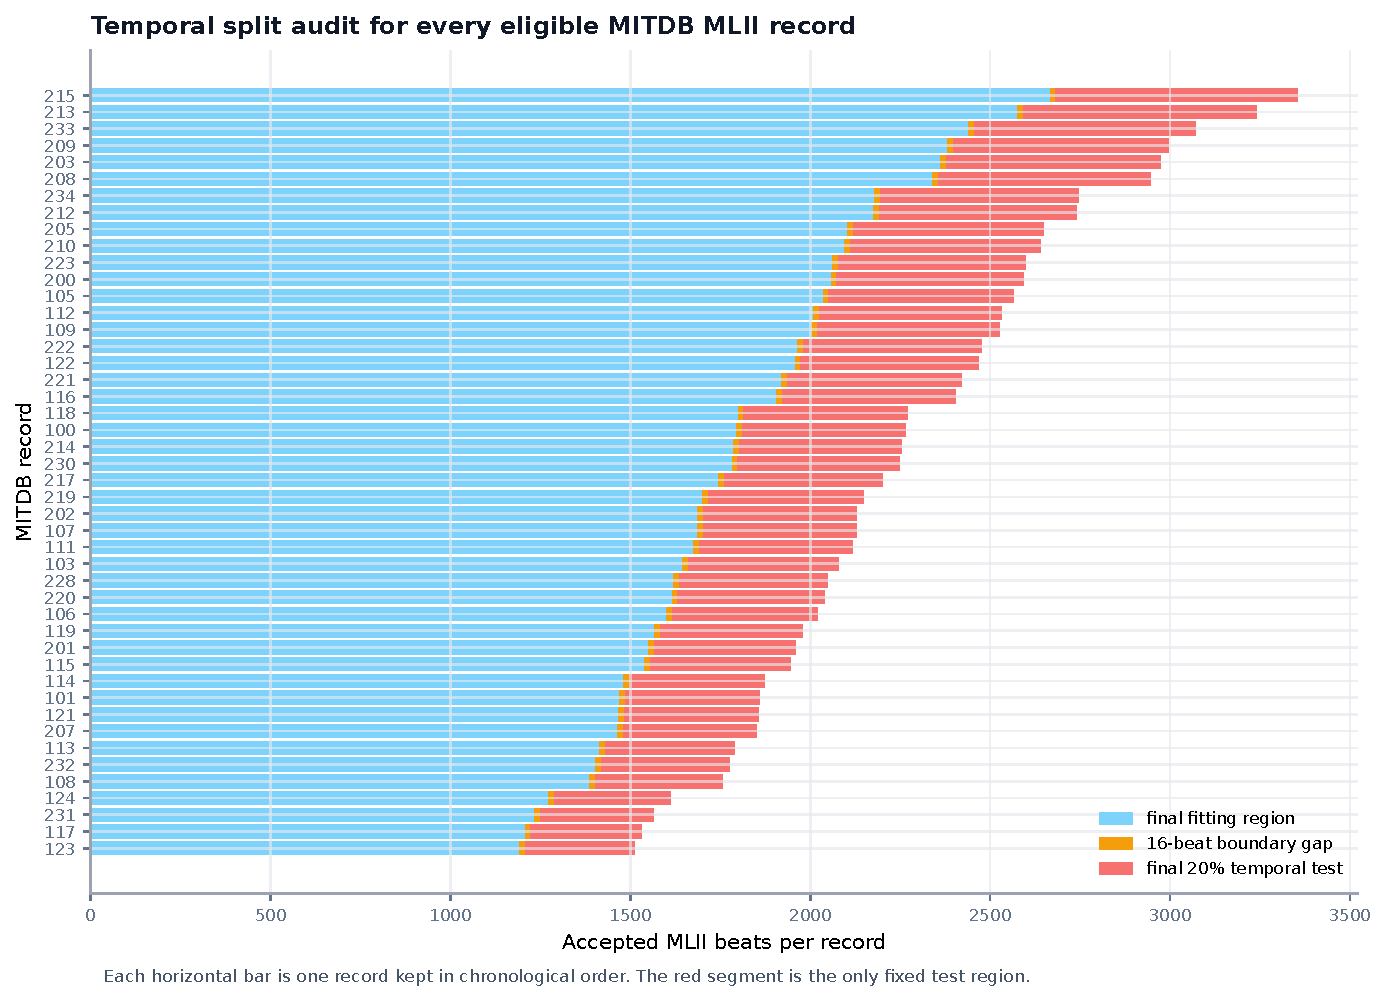
\includegraphics[width=.98\textwidth,height=.70\textheight,keepaspectratio]{pic/generated/method_temporal_split_audit.pdf}
\caption{Temporal split audit for every eligible MITDB MLII record. Blue beats
are available for final fitting, yellow beats are the boundary gap before the
test, and red beats are the held-out final 20\% temporal test.}
\label{fig:method-split-audit}
\end{figure}

The final held-out test contains 20,969 accepted beats. These are later beats
from known patients, not beats from unseen patients. The method prevents signal
overlap across the test boundary, but it intentionally keeps patient overlap.

\subsection{Model selection and final fitting}

Model selection uses only the earlier temporal validation region. In this
rerun, the final 20\% test region does not choose the candidate, threshold, or
hyperparameters.

Three binary Extra Trees candidates were fitted on the earlier candidate
region and ranked by validation balanced accuracy, then by F1. Three subtype
Extra Trees candidates were fitted only on supported abnormal candidate beats
and ranked by validation macro F1, then by accuracy. Figure~\ref{fig:method-model-selection}
shows the validation scores that selected the final pair.

The candidate-fitting rows, validation rows, sample weights, and final refit
are defined mathematically in Section~\ref{sec:method-training-inference}.
After selection, the binary model was refitted on all 83,050 eligible
development beats and the subtype model on 28,758 supported abnormal
development beats. The selected threshold was retained. Thus validation
measures model-selection performance, while the final temporal segment
measures the frozen refits under the stated retrospective protocol.

\begin{figure}[H]
\centering
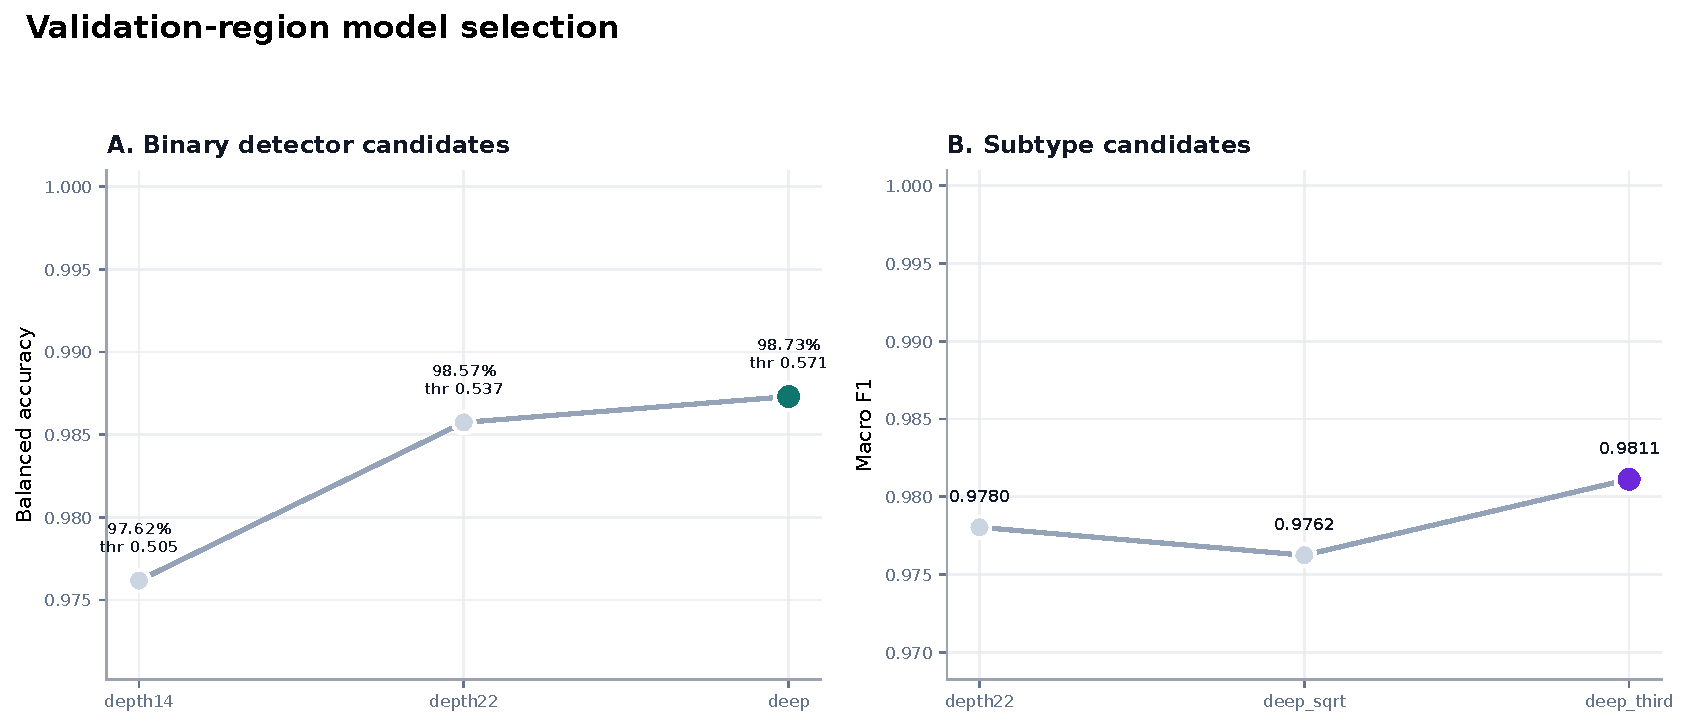
\includegraphics[width=.98\textwidth]{pic/generated/method_model_selection.pdf}
\caption{Model selection on the 64--80\% validation region. The binary detector
is selected by balanced accuracy and F1; the subtype classifier is selected by
macro F1 and accuracy.}
\label{fig:method-model-selection}
\end{figure}

The selected binary detector was the fully grown 240-tree candidate with
square-root feature sampling, minimum leaf size one, and record-weighting
power 0.35. Its validation-selected abnormal threshold was 0.5708333. The
selected subtype classifier was the fully grown 260-tree candidate with
a feature-sampling fraction of 0.33, minimum leaf size one, and record-weighting power
0.25. After selection, the binary model was refitted on all development beats,
whereas the subtype model was refitted only on supported abnormal development
beats.

\subsection{Evaluation order}

The three evaluation populations answer different questions about the
hierarchy defined in Section~\ref{ch:architecture}.

\begin{figure}[H]
\centering
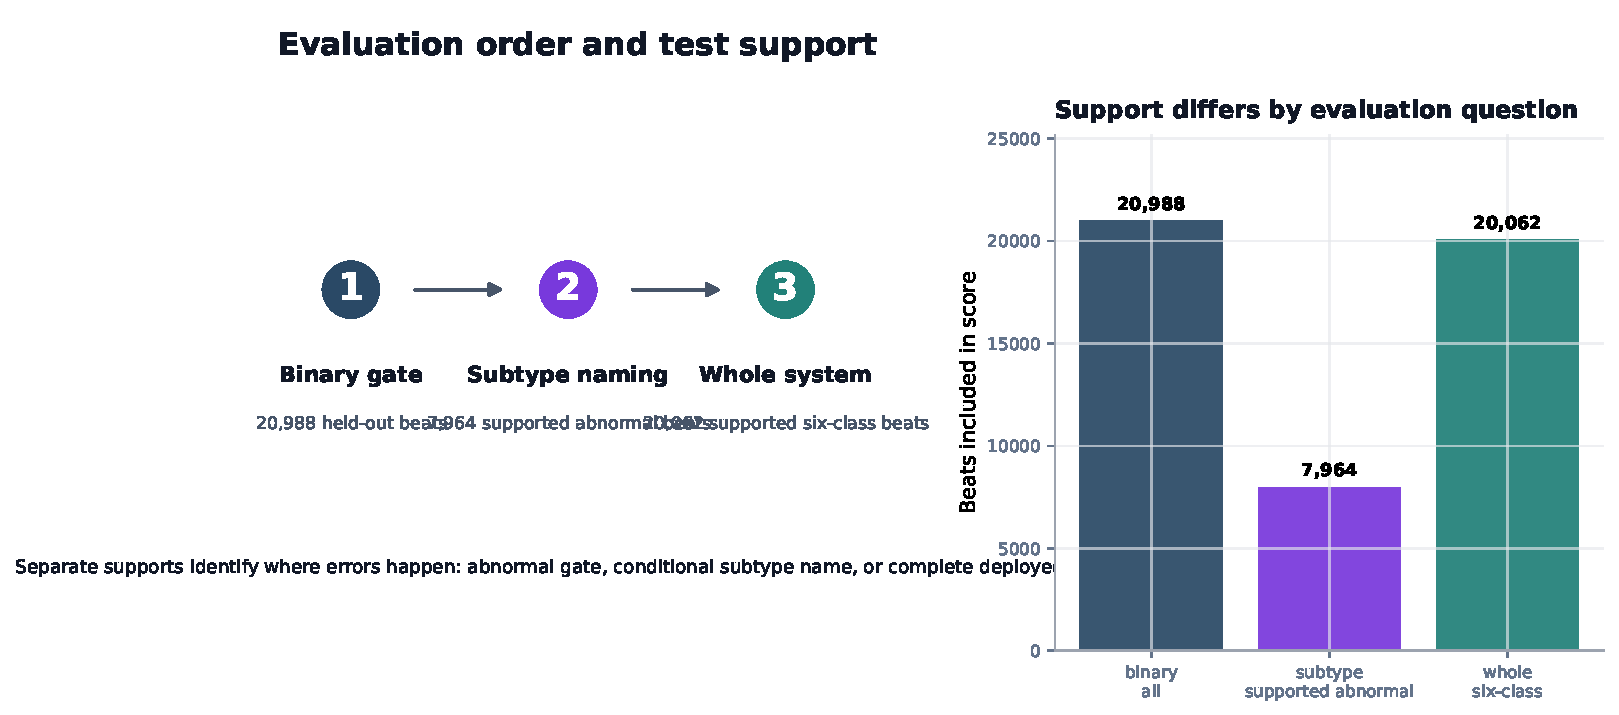
\includegraphics[width=.98\textwidth]{pic/generated/method_evaluation_order.pdf}
\caption[Populations used for the three evaluation questions.]{Populations used
for the three evaluation questions. Conditional subtype scoring uses true
supported abnormal beats independently of the gate. Complete-system scoring
uses the gate and subtype model together. The populations overlap; unsupported
abnormal labels enter only the binary evaluation.}
\label{fig:method-evaluation-order}
\end{figure}

The temporal evaluation uses three sets of beats:
\begin{enumerate}
    \item binary abnormality detection on all 20,969 held-out beats, including
    unsupported abnormal MITDB symbols;
    \item conditional subtype classification on 7,958 true supported abnormal
    beats; and
    \item whole-system N/PVC/PAC/LBBB/RBBB/AFib classification on 20,043
    supported held-out beats.
\end{enumerate}
The 926 unsupported abnormal beats are useful for testing the binary
normal/abnormal gate, but they are not scored in the six-class whole-system
confusion matrix.

\subsection{Limited external evaluation protocol}\label{sec:external-protocol}

After model fitting, the fixed hierarchy and threshold were applied to
complete INCART records I01 and I02. These were the two lead-II recordings
already cached locally at the start of the external evaluation. Selection was by local
availability, not measured performance. This is a convenience sample.
INCART contains 75 half-hour records from 32 source patients, with 12 leads
sampled at 257 Hz \cite{incartdb}. I01 and I02 both carry the header identifier
\emph{patient 1}: the two records represent one independent source patient.

Standard lead II is a practical external counterpart to MITDB MLII, not an
identical lead. This check combines source, acquisition and lead differences.
Scoring uses annotated beats, not live R-peak detections.

No external labels were used to refit the models or adjust the threshold.
The result is an exploratory transfer check; one source patient cannot
support a patient-cluster population confidence interval. Performance is
reported in Section~\ref{sec:external-incart}.

\subsection{Metrics}

For binary detection, an abnormal beat is the positive class. $TP$ and $TN$
are correctly classified abnormal and N beats; $FP$ is an N beat predicted
as abnormal, and $FN$ is an abnormal beat predicted as N. The metrics are
\begin{align}
 \mathrm{Accuracy}&=\frac{TP+TN}{TP+TN+FP+FN},\\
 \mathrm{Sensitivity}&=\frac{TP}{TP+FN},\\
 \mathrm{Specificity}&=\frac{TN}{TN+FP},\\
 \mathrm{Balanced\ accuracy}&=\frac{\mathrm{Sensitivity}+\mathrm{Specificity}}{2}.
\end{align}
For each output class $c$, the remaining classes are treated as negative
when calculating
\begin{align}
 \mathrm{Precision}_c&=\frac{TP_c}{TP_c+FP_c},\\
 \mathrm{Recall}_c&=\frac{TP_c}{TP_c+FN_c},\\
 F1_c&=\frac{2\,\mathrm{Precision}_c\mathrm{Recall}_c}
 {\mathrm{Precision}_c+\mathrm{Recall}_c}.
\end{align}
Macro F1 is the unweighted mean of class F1 values. It gives PAC the same
weight as N even though N contains many more beats. The saved scoring code
assigns zero when a precision, recall, or F1 denominator is zero. A class
with no reference examples still has no empirically estimable sensitivity;
the numerical convention does not supply evidence about that class.

Two accuracy summaries are reported. Pooled beat accuracy gives every beat
equal weight. Equal-subject accuracy first calculates accuracy within each of
the 45 eligible subject clusters and then gives every subject equal weight:
\begin{equation}
 A_{macro}=\frac{1}{45}\sum_{s=1}^{45}A_s.
 \label{eq:subject-macro}
\end{equation}
The equal-subject mean is used for uncertainty analysis so that subjects
with more beats do not receive more weight. For conditional subtype accuracy,
only subjects with supported abnormal test beats have a defined score; the
mean uses that smaller set of subjects.

\subsection{Subject-clustered confidence interval}

The primary 95\% confidence interval uses a non-parametric percentile
bootstrap:
\begin{enumerate}
    \item keep every beat from one subject together;
    \item treat records 201 and 202 as one subject cluster;
    \item sample 45 subject clusters with replacement;
    \item calculate the equal-subject mean accuracy;
    \item repeat 10,000 times using seed 20260801; and
    \item take the 2.5th and 97.5th percentiles.
\end{enumerate}
For conditional subtype accuracy, a sampled cluster without supported
abnormal test beats has an undefined score and is omitted from that
replicate's mean. The resampling still draws from all 45 clusters; the
number of defined subtype scores can therefore vary between replicates.
These intervals describe variation across the evaluated subject clusters with
the fitted model held fixed. They do not include retraining variability,
uncertainty from earlier test exposure, or a new population shift.
Resampling individual beats can create an artificially narrow interval
because adjacent beats from the same recording are correlated. The clustered
bootstrap keeps that dependence \cite{rutter2000clustered}.

\subsection{Exploratory tests against the 90\% target}

The confidence interval is the primary statistical evidence. Two
non-parametric tests provide supplementary, exploratory analyses. The exact one-sided sign
test asks whether more than half of subjects exceed 90\%. The one-sided
Wilcoxon signed-rank test asks whether subject accuracies are shifted above
90\%, under the additional symmetry assumption of a signed-rank location
test. Accuracy is bounded and has ceiling effects, so the Wilcoxon analysis is
secondary. The sign test concerns the fraction of subjects above the target,
not pooled beat accuracy. These tests are interpreted together with the confidence interval,
interval width, per-class recall, macro F1, and subject accuracy distribution.

\subsection{Reproducibility and leakage controls}

The final experiment saves the temporal boundary audit for every record, the
candidate scores, selected models, probability threshold, final confusion
matrix, per-class counts, per-subject accuracies, bootstrap seed, and headline
metrics. The rerun used seed 20260801 and did not use the final 20\% segment
for candidate selection, threshold selection, or final refitting.

The final 20\% segment had been observed during earlier system development, so
the evaluation is a retrospective rerun on previously observed data.
This prior exposure can influence design choices and cause optimism even
when the present selection code excludes test rows. It is not a confirmatory
first-use test, and the bootstrap does not correct development-selection bias. Patient overlap is
also intentional: the test is later ECG from known patients. Therefore, the
method supports a patient-adapted temporal-performance claim, not a
patient-independent generalisation claim.

